\subsection{Результаты моделирования}

Оценивалась работа вариантов алгоритма. Различаются они в
вопросе выбора следующей целевой точки перемещения юнита:
\begin{mintemize}
\item случайный выбор
\item поиск ближайших неизведанных зон
\item равномерное распределение по карте
\end{mintemize}

Как критерий оценки использовалось состояние карты на момент
времени $T$ работы системы. В состояние карты входят:

\begin{mintemize}
\item соотношение количества известных секторов к общему
\item средняя разница между последней проверкой и текущим временем
    для известных секторов карты
\end{mintemize}

Для каждого алгоритма было произведено 3 эксперимента с разным
количеством юнитов: 16, 33, 50. Моделируемое время составляло
$\approx 60\text{сек}$. Юниты начинали движение из области над
центром карты.

Графики строились в программе \verb|gnuplot|, информация для
построения генерировалась ПМО.

\newpage
\subsubsection{Случайный выбор}

Самый простой в реализации и логике вариант алгоритма разведки
местности. Новая целевая точка выбирается случайным образом в
пределах карты.

\begin{figure}[h!]
    \centering
    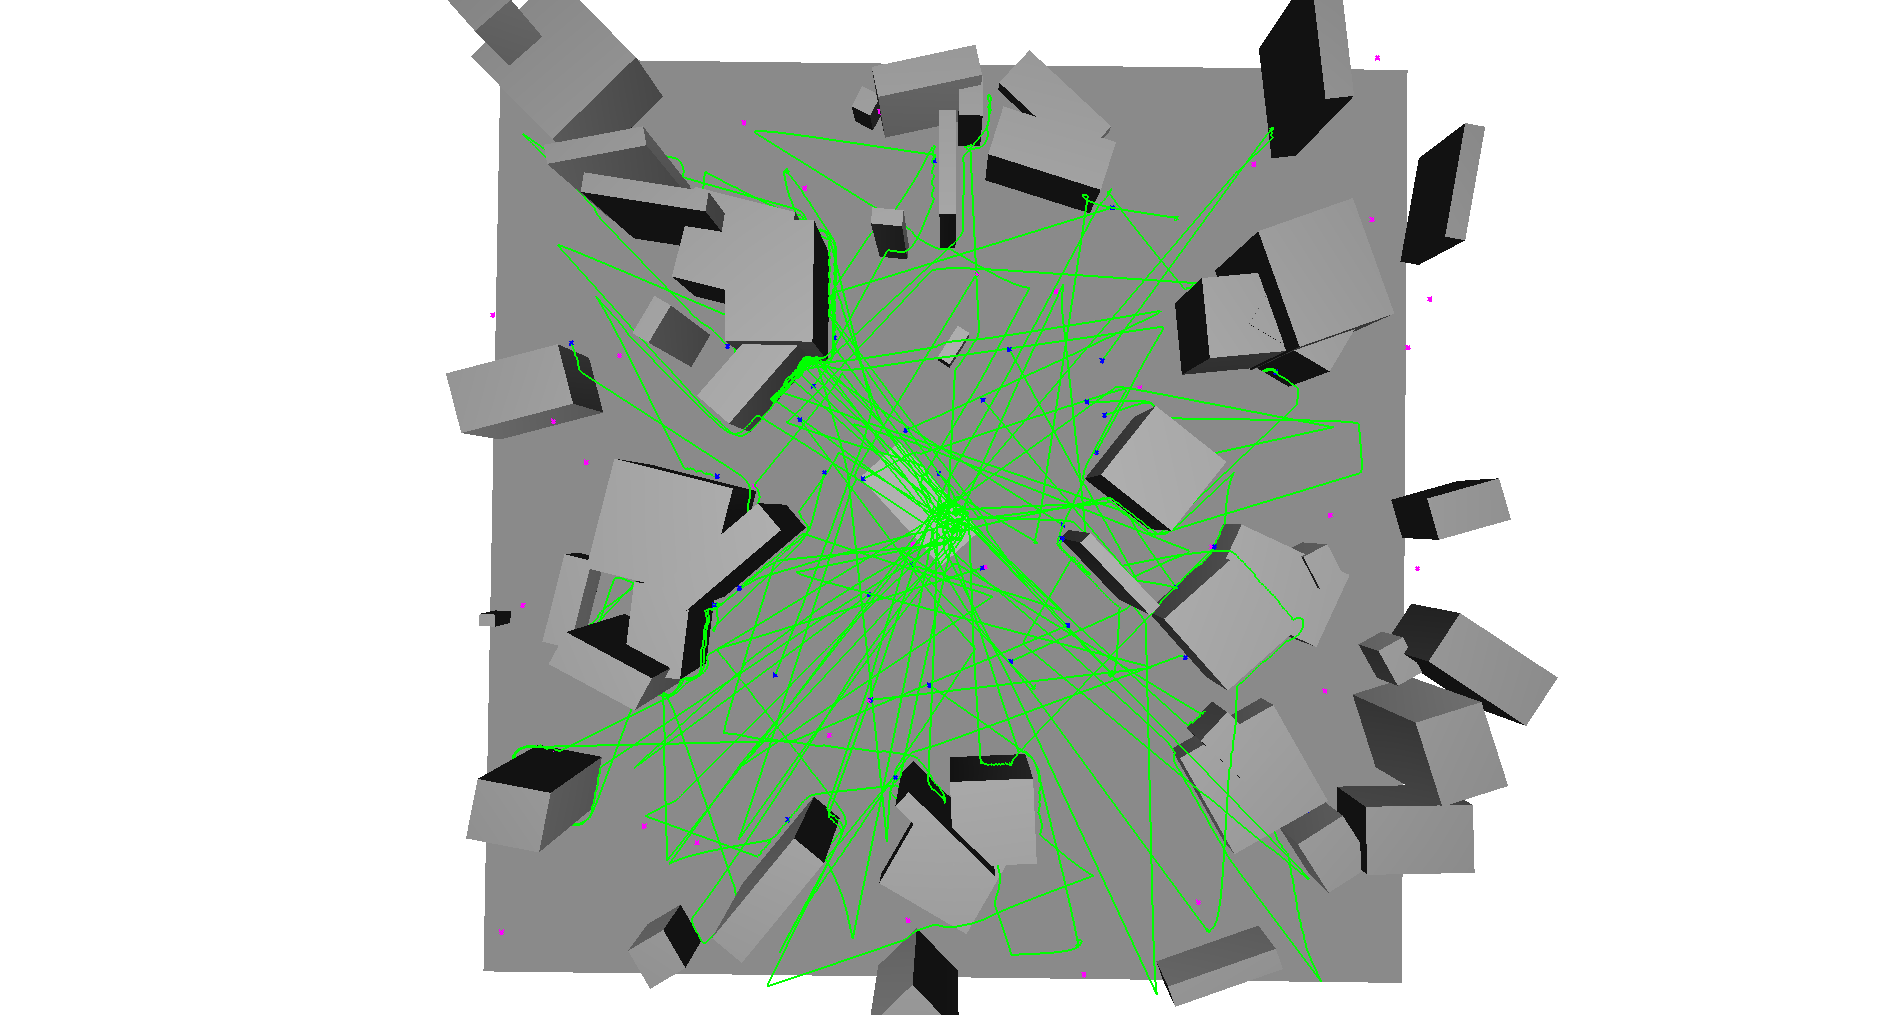
\includegraphics[width=\linewidth]{s50rm_view.png}
    \caption{Случайный выбор, 50 юнитов, вид сверху, пути перемещения}
    \label{fig:s50rm_view}
\end{figure}

На рис. \ref{fig:s50rm_view} зелёными линиями отображены маршруты перемещения юнитов 
по местности.

\begin{figure}[h!]
    \centering
    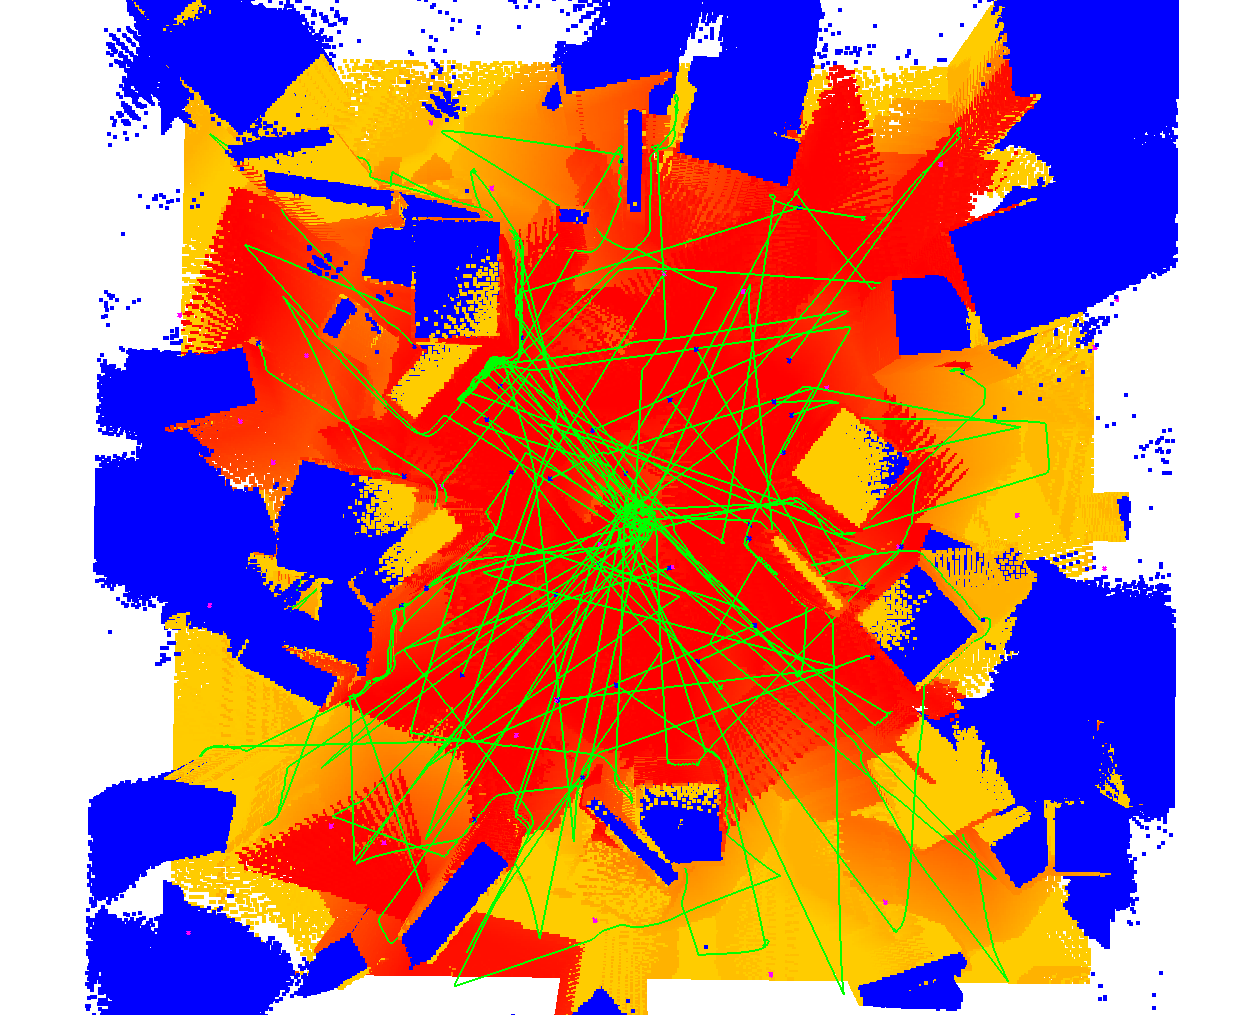
\includegraphics[width=\linewidth]{s50rm_map.png}
    \caption{Случайный выбор, 50 юнитов, вид сверху, состояние карты}
    \label{fig:s50rm_map}
\end{figure}

На рис. \ref{fig:s50rm_map} синим цветом отмеченны неизведанные области, красным --
только что обновлённые сектора, жёлтым -- "устаревшие". Данные цветовые обозначения
используются для всех последующих снимков интерфейса симулятора.

\begin{figure}[h!]
    \centering
    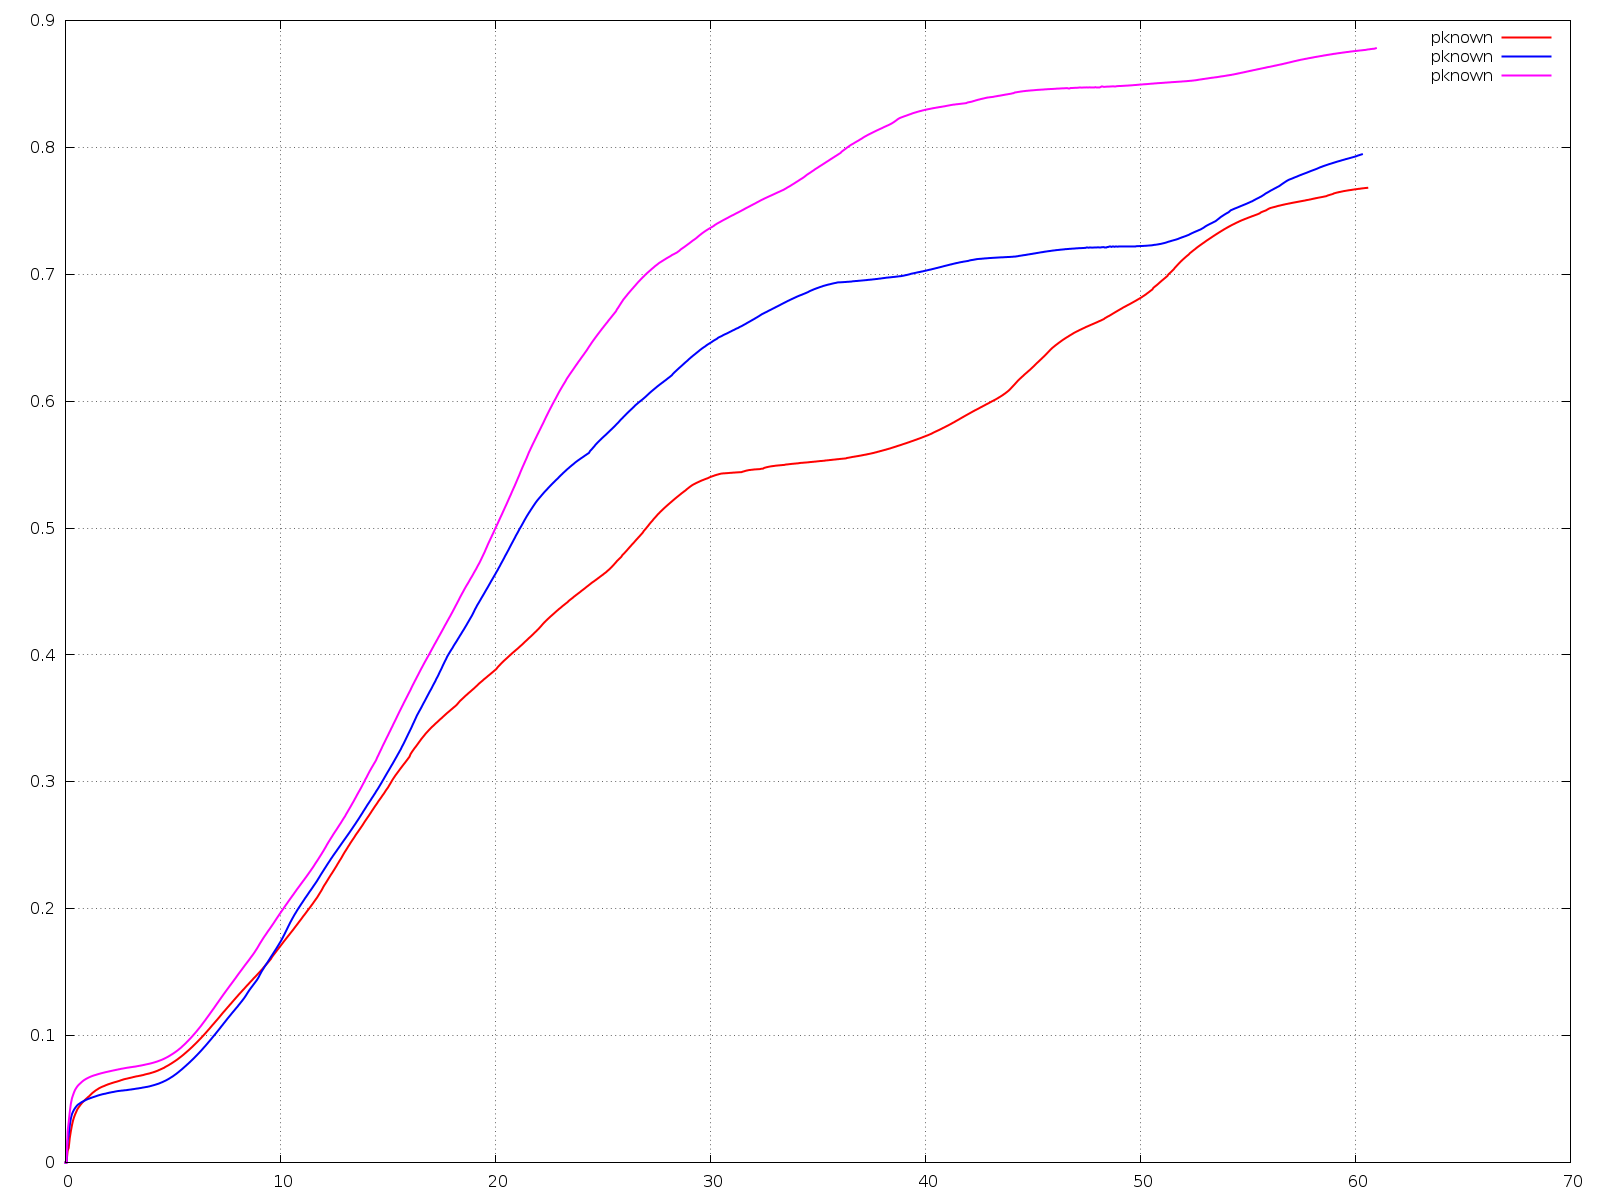
\includegraphics[width=.9\linewidth]{all_rnd_auto_pknown.png}
    \caption{Случайный выбор, 3 эксперимента, количество изведанных секторов от времени}
    \label{fig:all_rnd_auto_pk}
\end{figure}

На рис. \ref{fig:all_rnd_auto_pk} показаны результаты оценки работы варианта алгоритма для
критерия соотношения изведанных секторов к общему количеству секторов карты в зависимости
от времени. Эксперименты отличаются количеством юнитов:
\begin{mintemize}
\item красный -- 16 юнитов
\item синий -- 33 юнита
\item зелёный -- 50 юнитов
\end{mintemize}

\begin{figure}[h!]
    \centering
    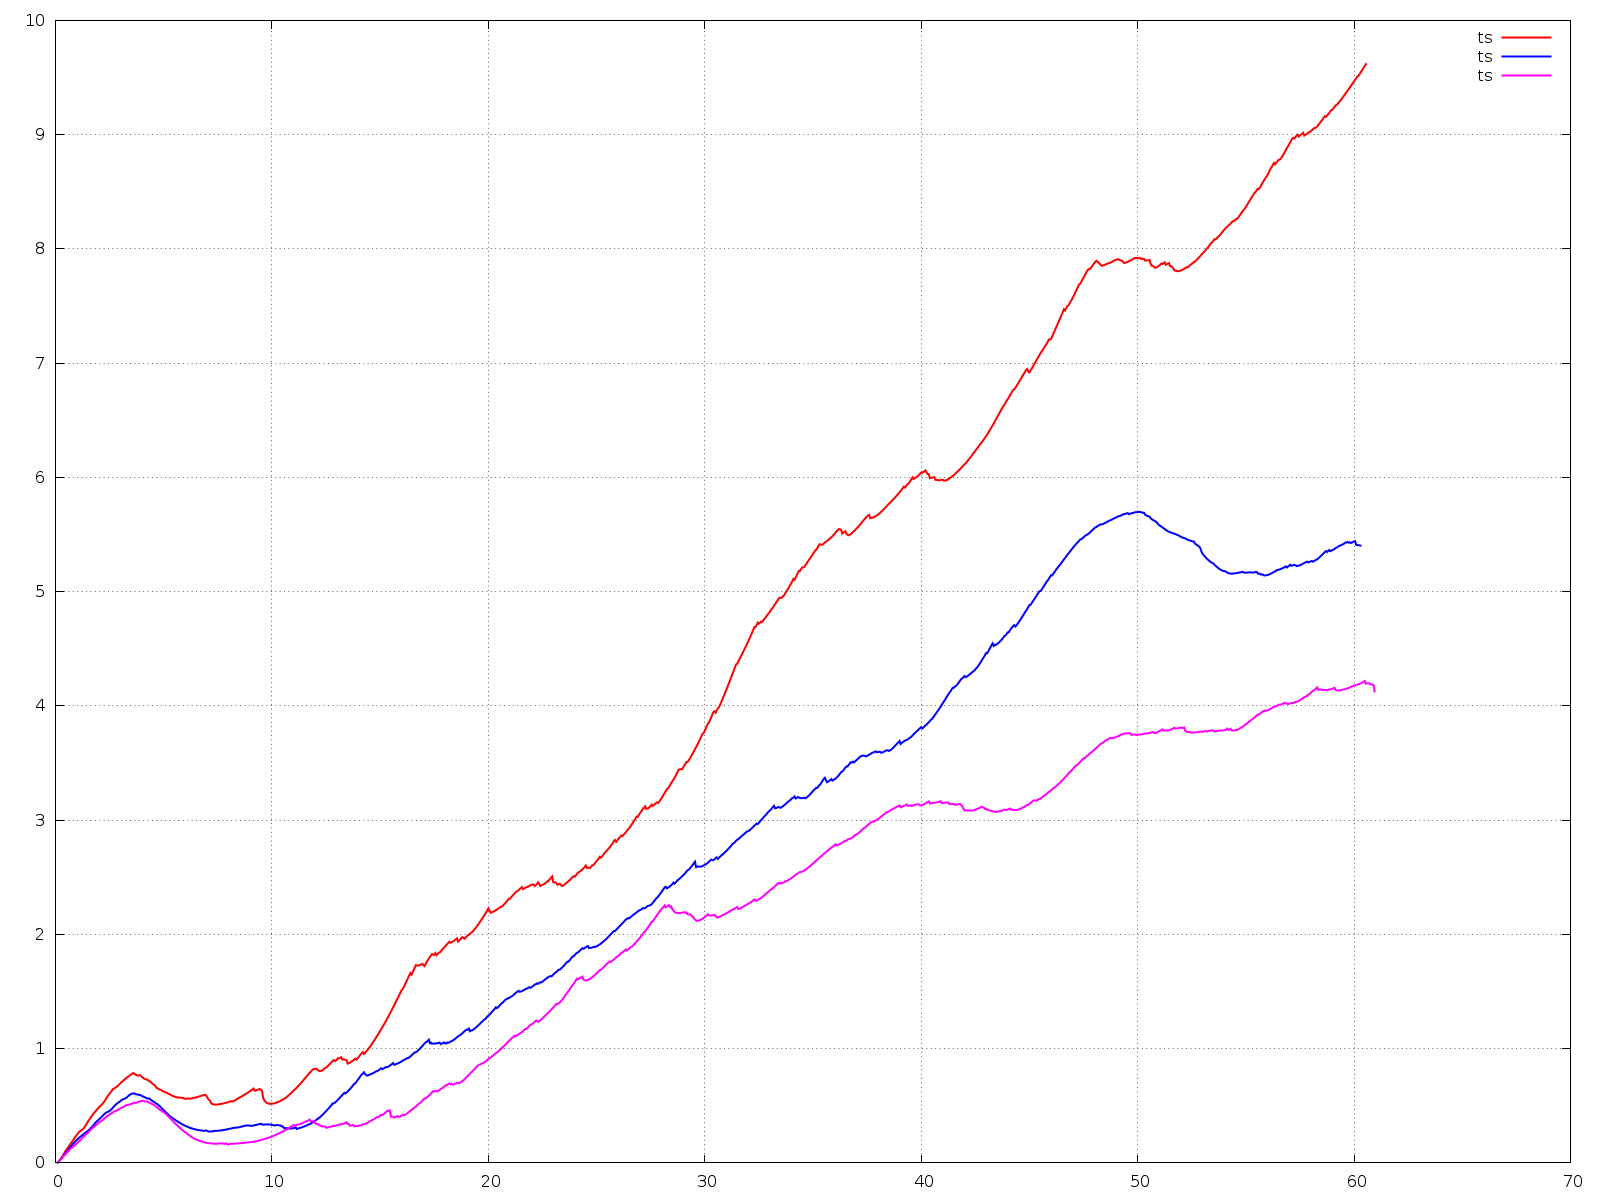
\includegraphics[width=.9\linewidth]{all_rnd_auto_ts.png}
    \caption{Случайный выбор, 3 эксперимента, интервал обновления от времени}
    \label{fig:all_rnd_auto_ts}
\end{figure}

\newpage

На рис. \ref{fig:all_rnd_auto_ts} показаны результаты оценки работы варианта алгоритма для
критерия разницы между временем последнего измерения и текущим временем.
Цветовая схема та же, что и для рис. \ref{fig:all_rnd_auto_pk}.

\clearpage
\newpage

\subsubsection{Поиск ближайших неизведанных зон}

Вариация алгоритма описана в секции \nnref{ref:algo:choise:find} (стр. \pageref{ref:algo:choise:find}).

\begin{figure}[h!]
    \centering
    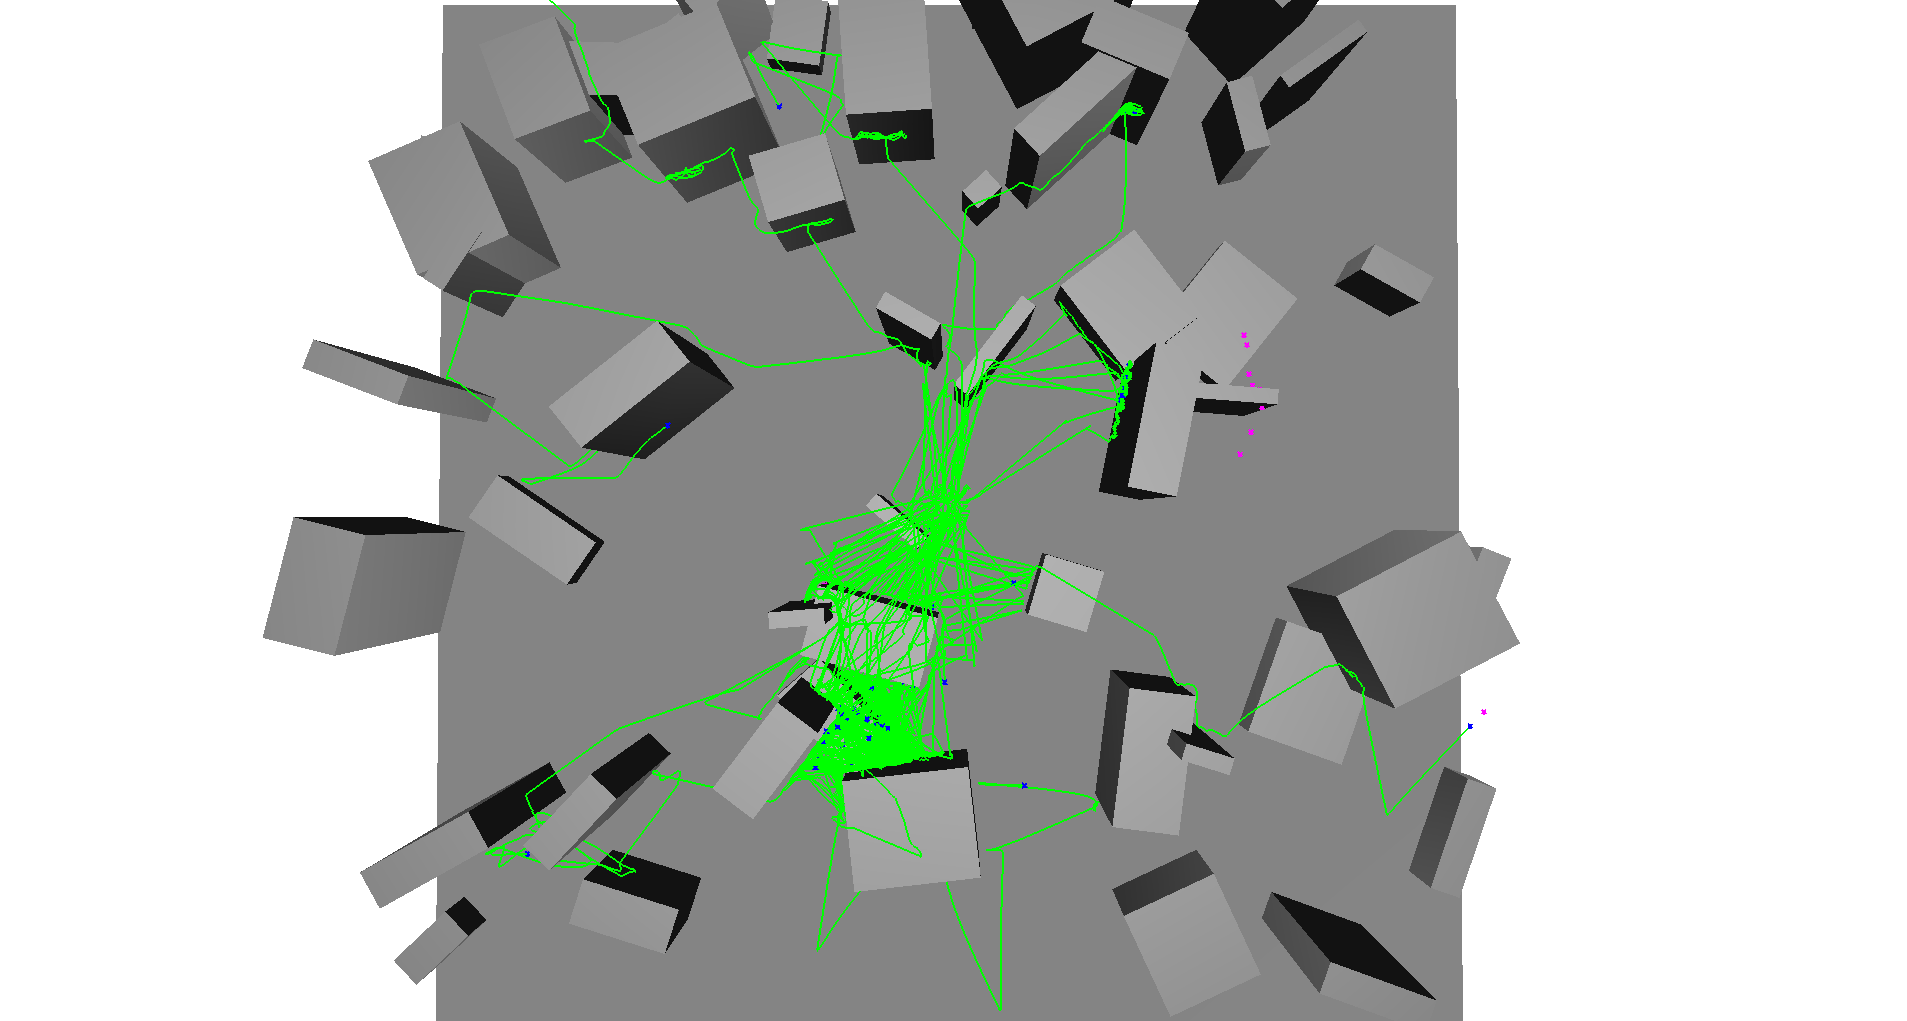
\includegraphics[width=\linewidth]{s50f4r_view.png}
    \caption{Поиск ближайших, 50 юнитов, вид сверху, пути перемещения}
    \label{fig:s50f4r_view}
\end{figure}

На рис. \ref{fig:s50f4r_view} можно заметить, что большое количество
юнитов собралось в одном месте. Такой результат объясняется отсутствием
учёта возможности доступа к целевой точке в этой вариации алгоритма.
В текущем случае каждая новая целевая точка для многих юнитов оказалась
внутри здания, в которое юниты не могут проникнуть.

\begin{figure}[h!]
    \centering
    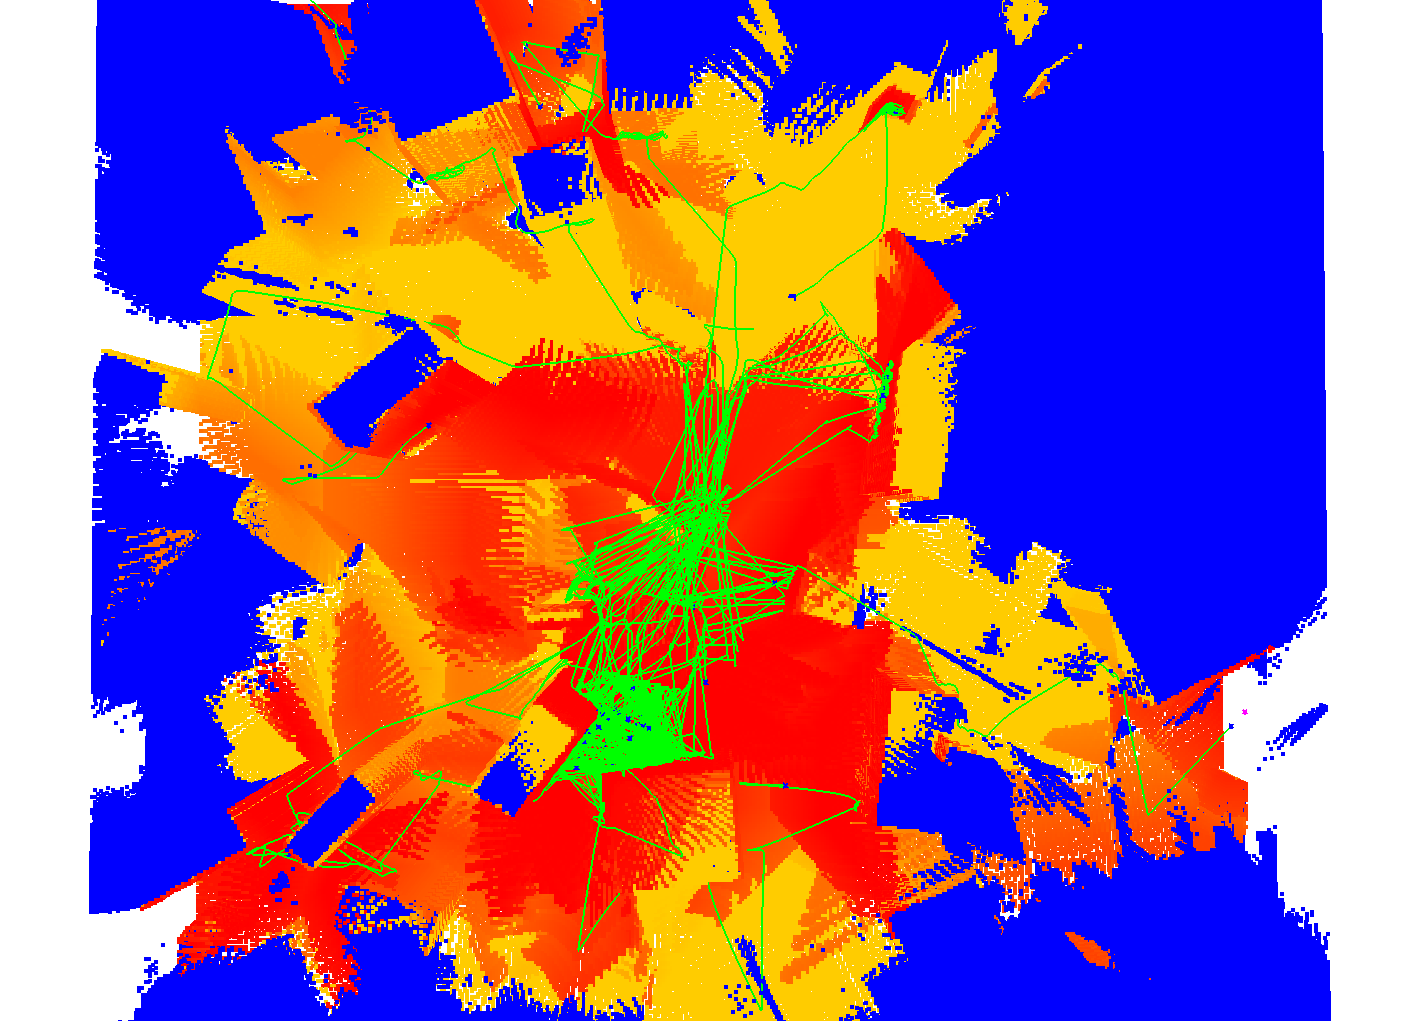
\includegraphics[width=\linewidth]{s50f4r_map.png}
    \caption{Поиск ближайших, 50 юнитов, вид сверху, состояние карты}
    \label{fig:s50f4r_map}
\end{figure}

На рис. \ref{fig:s50f4r_map} хорошо видно, что концентрация юнитов в
одном месте неблаготворно влияет как на разведывательную функцию МБПЛА,
так и на функцию наблюдения. Также к подобному выводу можно прийти,
анализируя графики на рис. \ref{fig:all_f4r_pk} и \ref{fig:all_f4r_ts}.

\begin{figure}[h!]
    \centering
    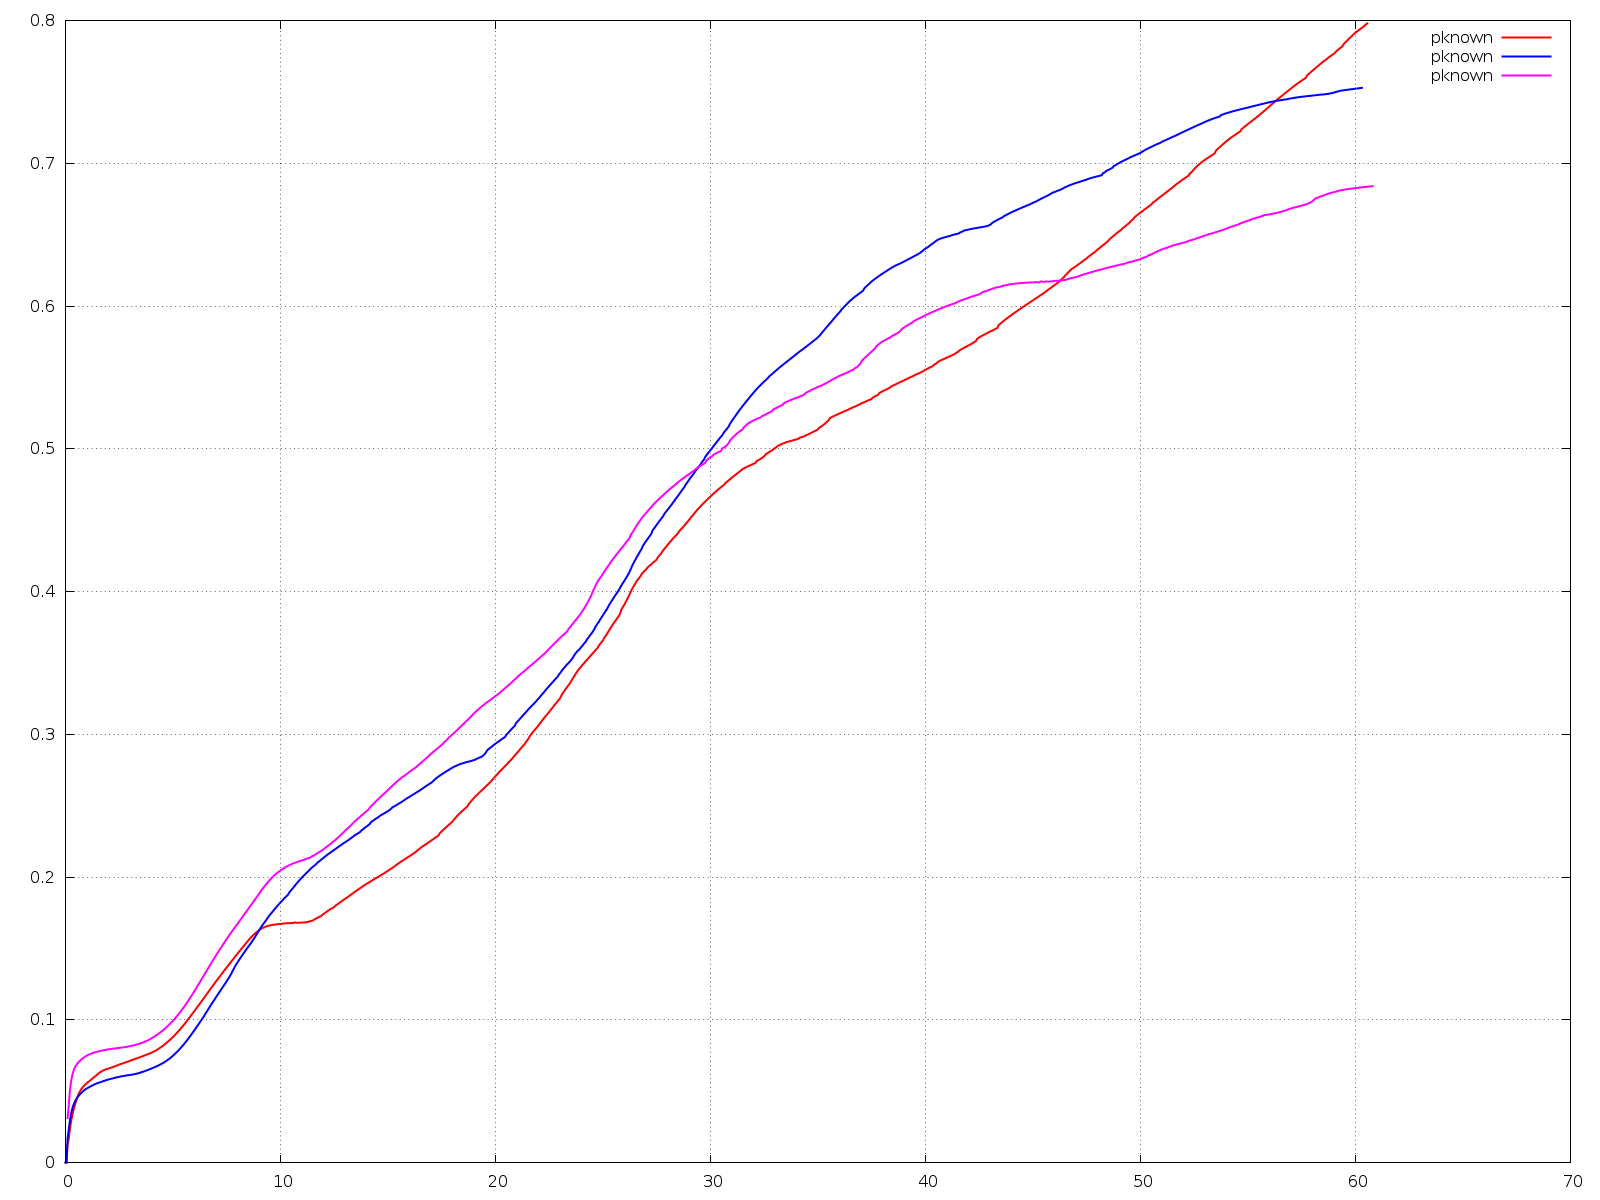
\includegraphics[width=.9\linewidth]{all_find_4_pknown.png}
    \caption{Поиск ближайших, 3 эксперимента, количество изведанных секторов от времени}
    \label{fig:all_f4r_pk}
\end{figure}

\clearpage

\begin{figure}[h!]
    \centering
    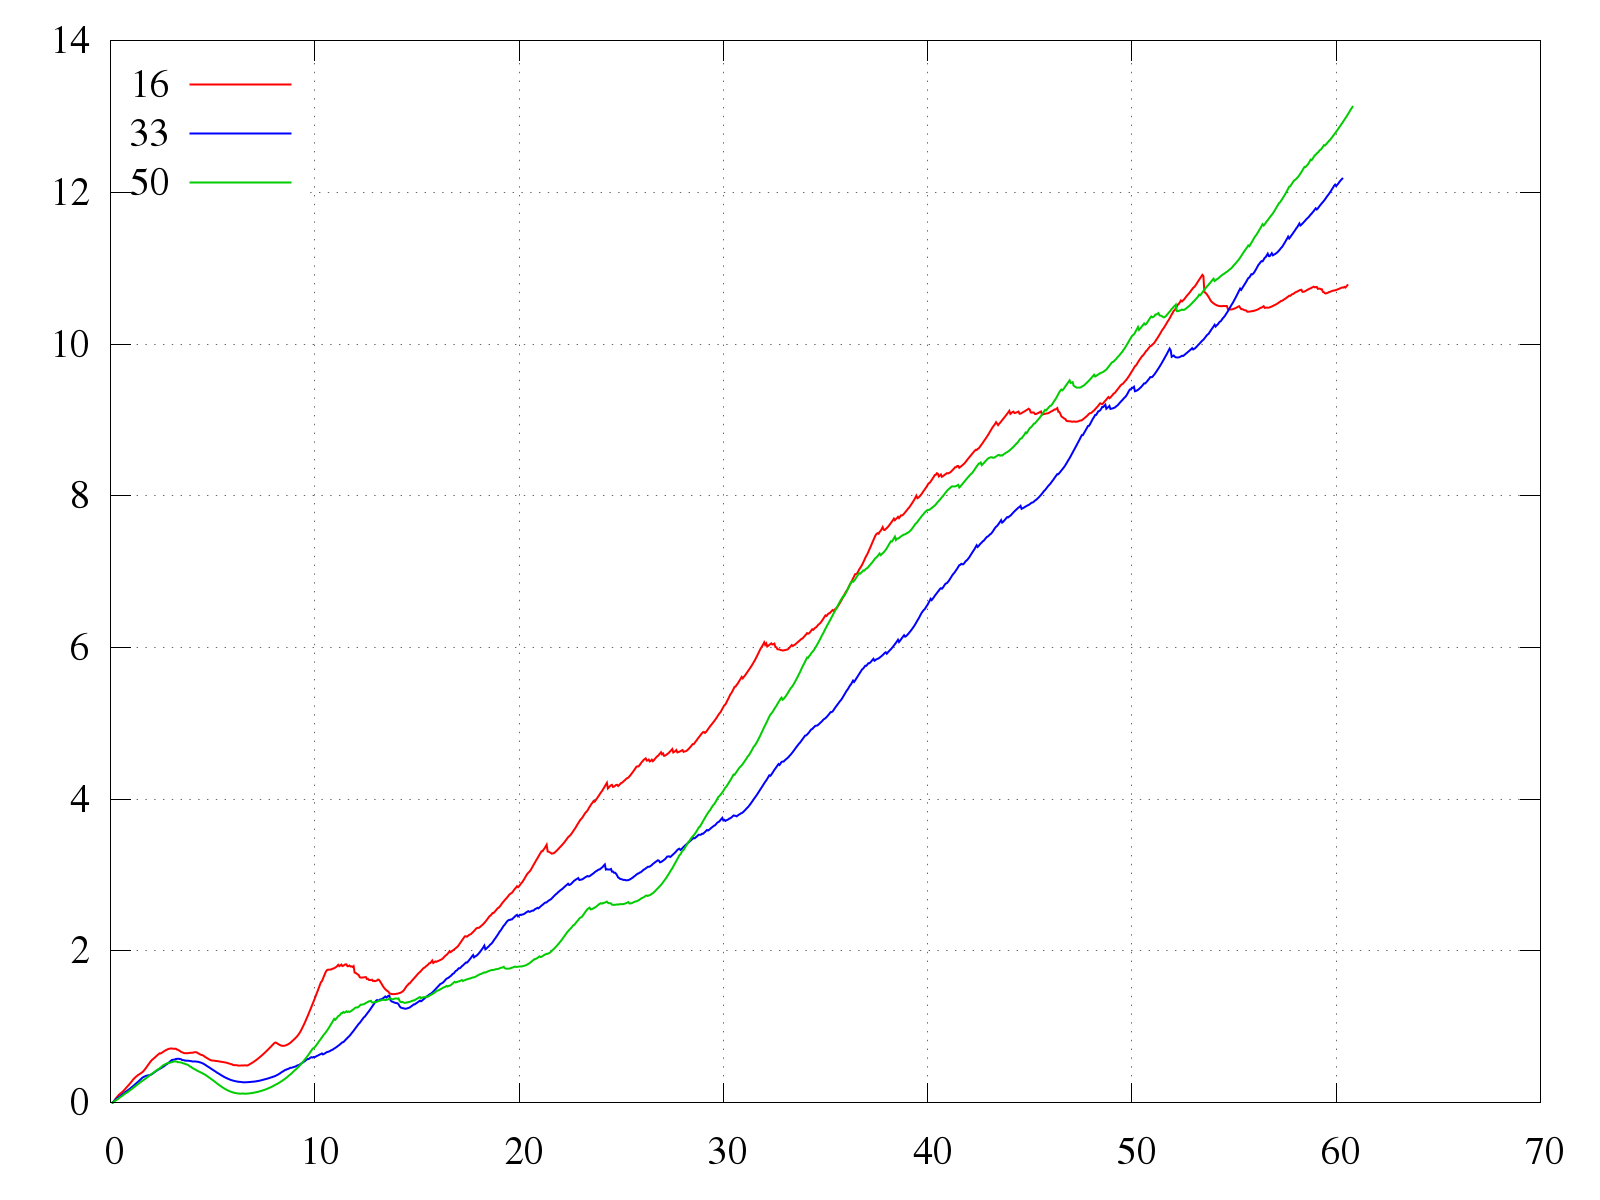
\includegraphics[width=.9\linewidth]{all_find_4_ts.png}
    \caption{Поиск ближайших, 3 эксперимента, интервал обновления от времени}
    \label{fig:all_f4r_ts}
\end{figure}

Из графиков на рис. \ref{fig:all_f4r_pk} и \ref{fig:all_f4r_ts} можно понять,
что данная вариация алгоритма одинаково плохо работает при разных количествах
юнитов.

\clearpage
\newpage

\subsubsection{Равномерное распределение по карте}

Юниты распределяются по регионам карты, в каждом регионе
оказывается примерно одинаковое поличество юнитов.

Вариация алгоритма описана в секции \nnref{ref:algo:choise:serial}
(стр. \pageref{ref:algo:choise:serial}).

\begin{figure}[h!]
    \centering
    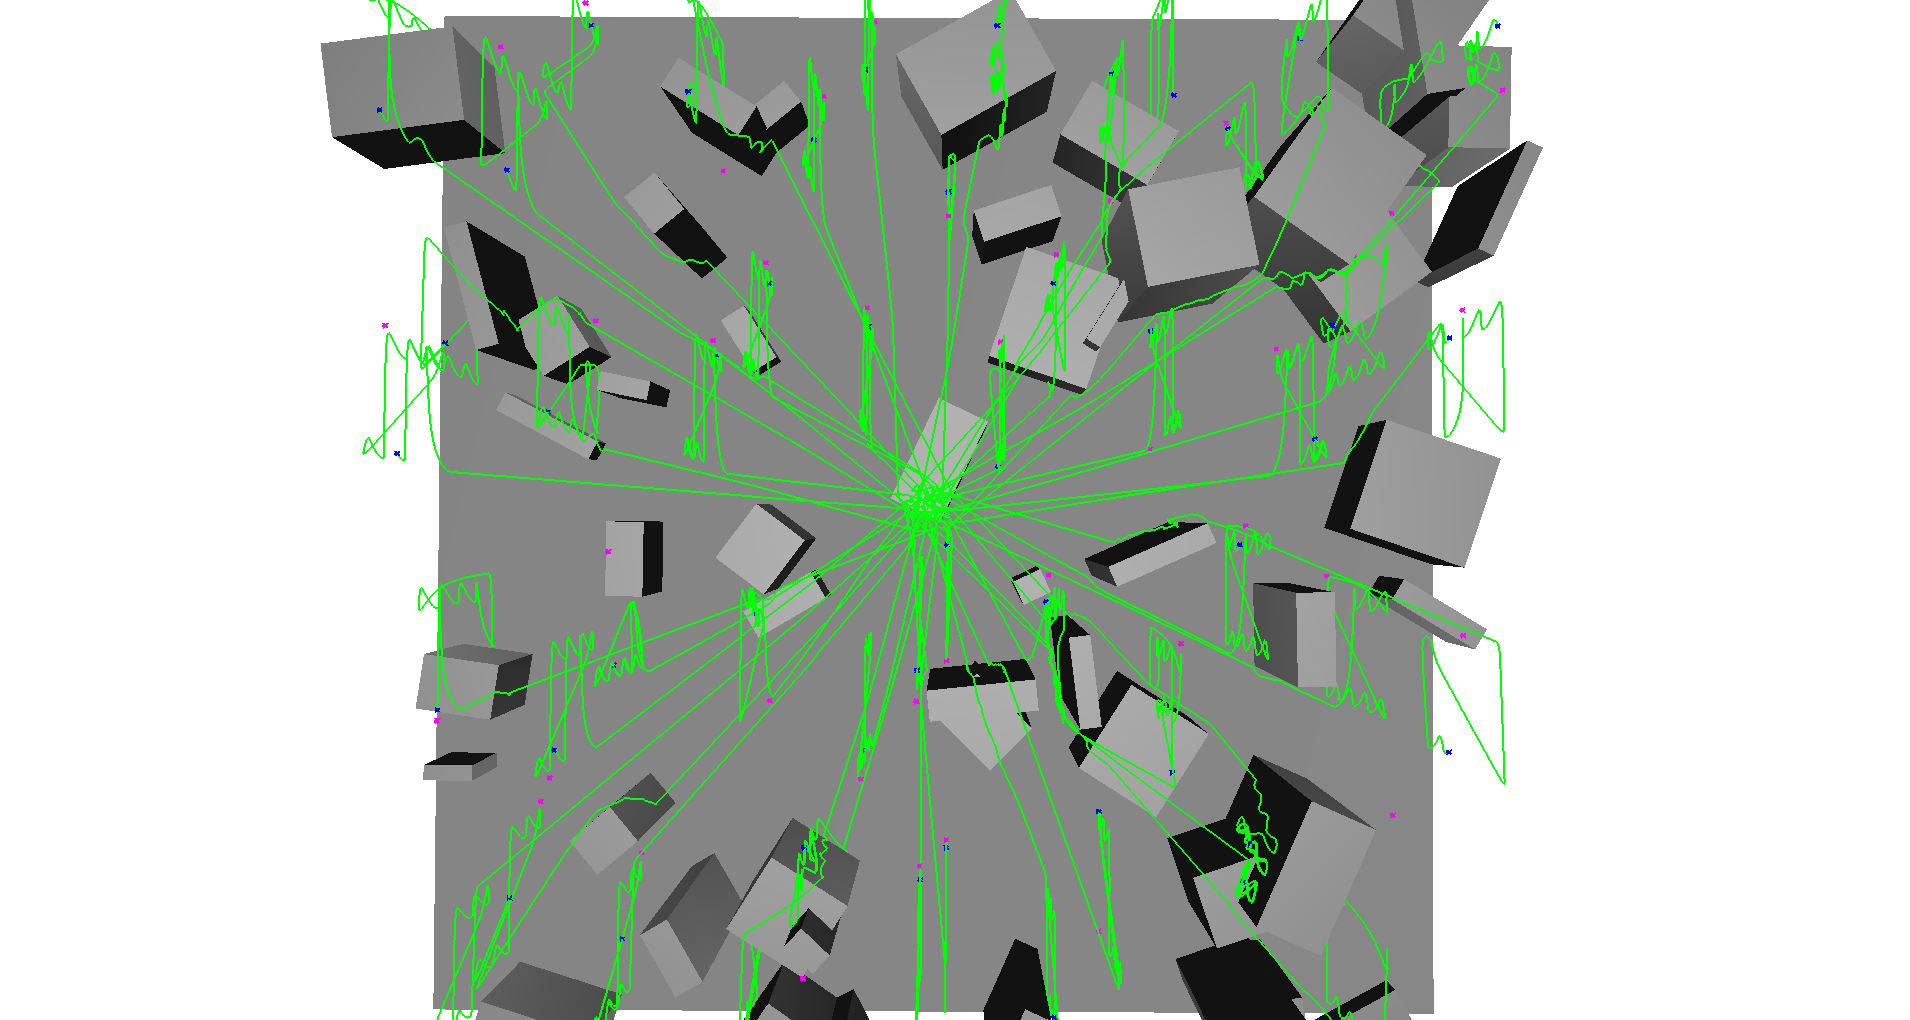
\includegraphics[width=\linewidth]{s50s_view.png}
    \caption{Равномерное распределение, 50 юнитов, вид сверху, пути перемещения}
    \label{fig:s50s_view}
\end{figure}

\begin{figure}[h!]
    \centering
    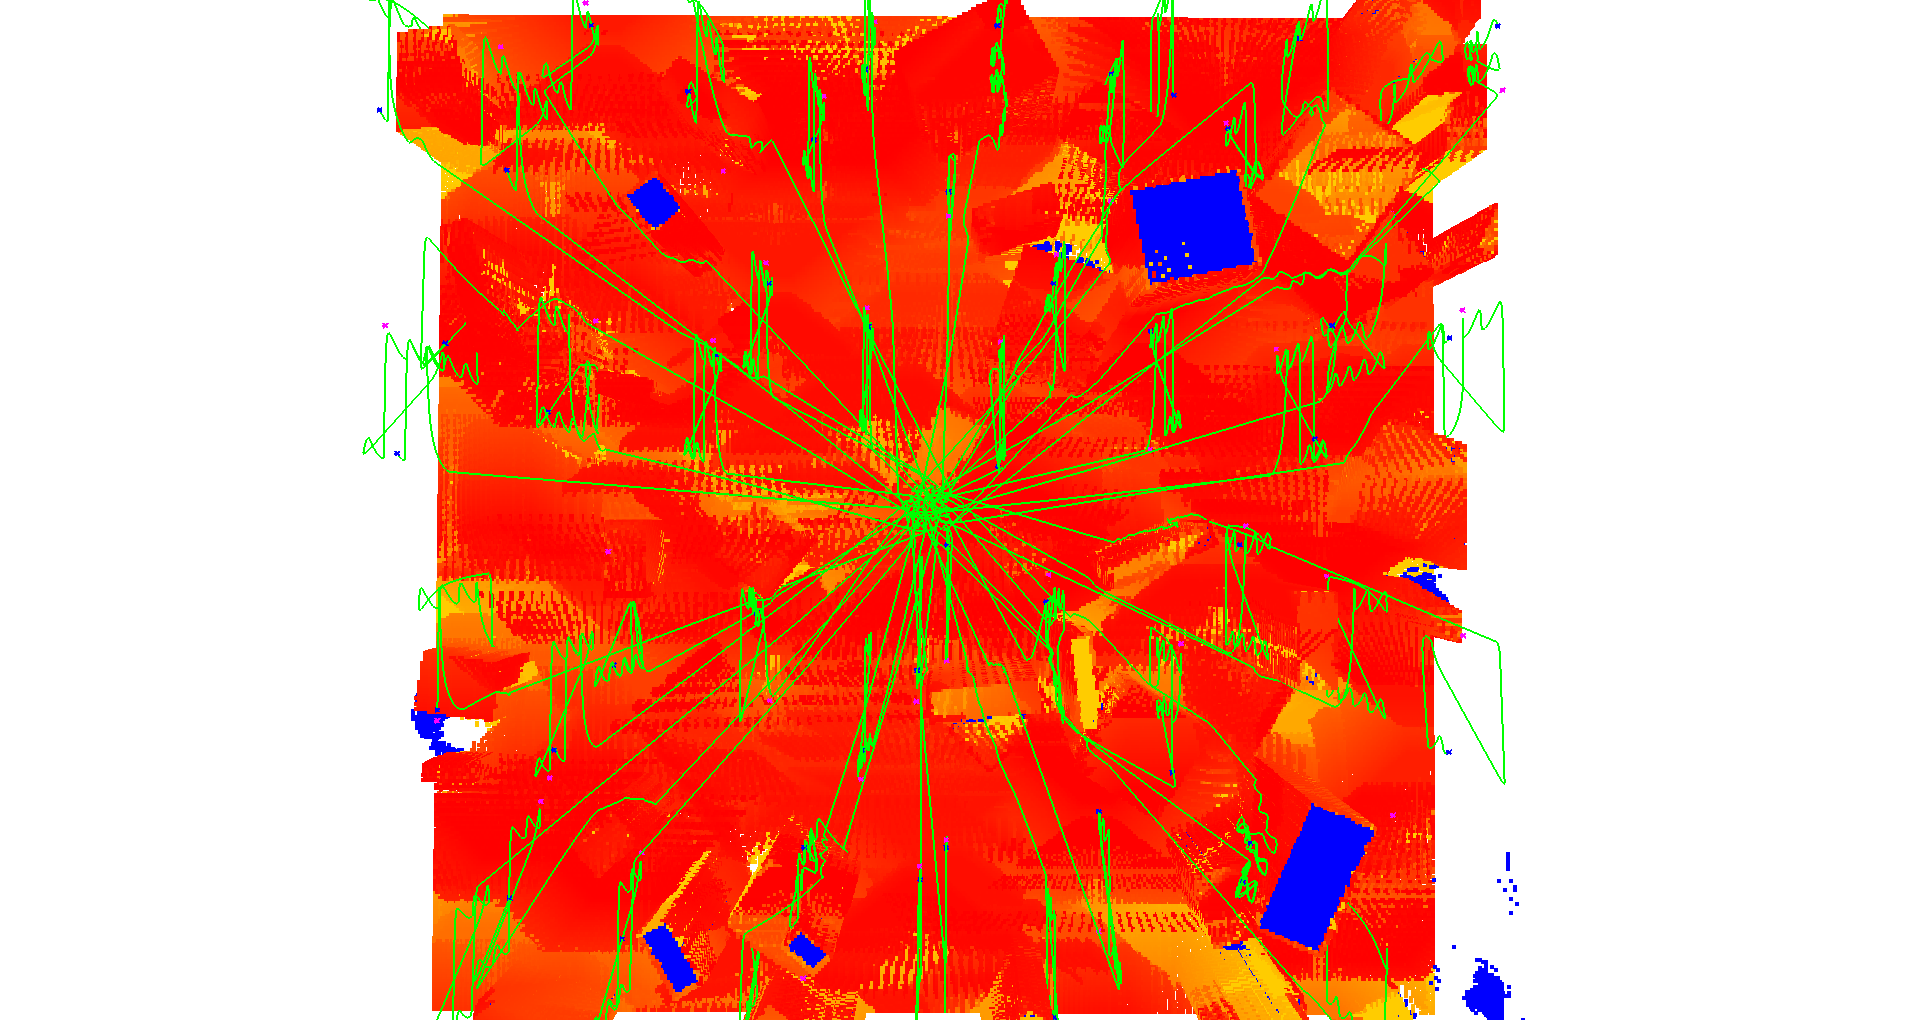
\includegraphics[width=\linewidth]{s50s_map1.png}
    \caption{Равномерное распределение, 50 юнитов, вид сверху, состояние карты}
    \label{fig:s50s_map1}
\end{figure}

По рисунку \ref{fig:s50s_map1} хорошо видно, что карта почти полностью известна, 
большая часть обновляется регулярно.

\begin{figure}[h!]
    \centering
    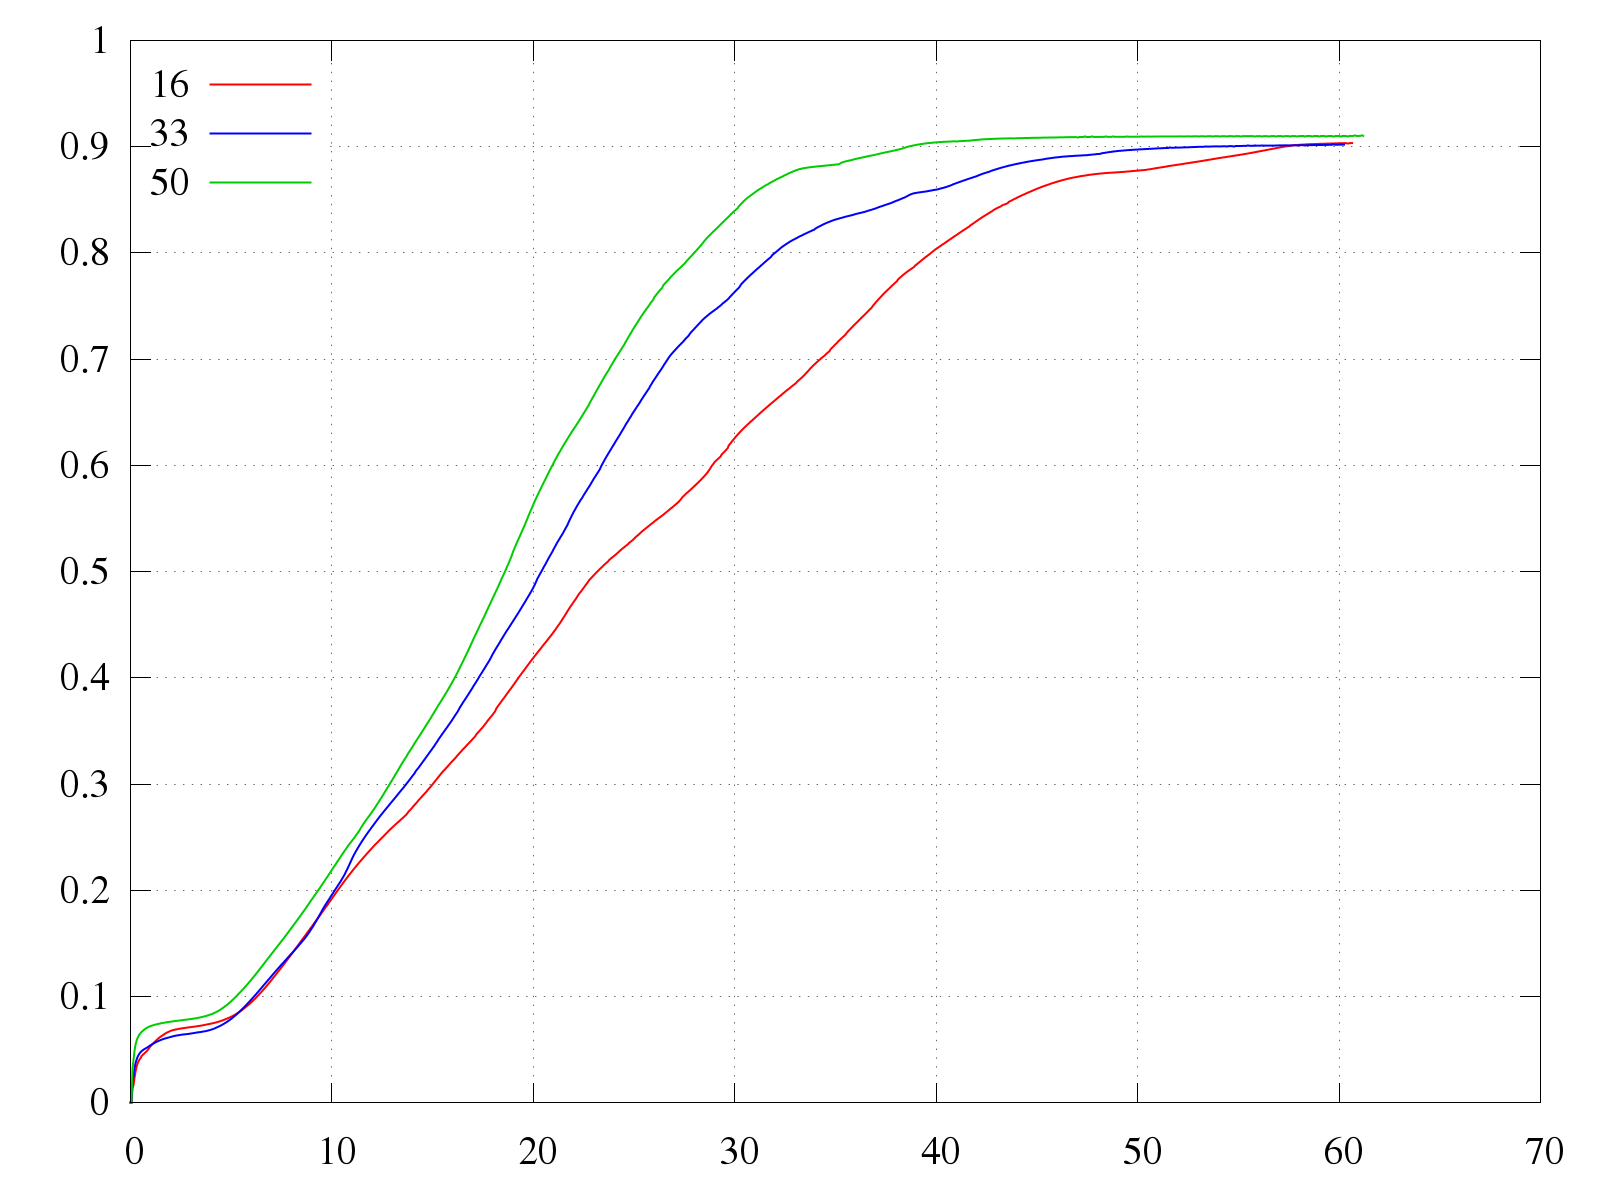
\includegraphics[width=.9\linewidth]{all_serial_pknown.png}
    \caption{Равномерное распределение, 3 эксперимента, количество изведанных секторов от времени}
    \label{fig:all_serial_pk}
\end{figure}

\begin{figure}[h!]
    \centering
    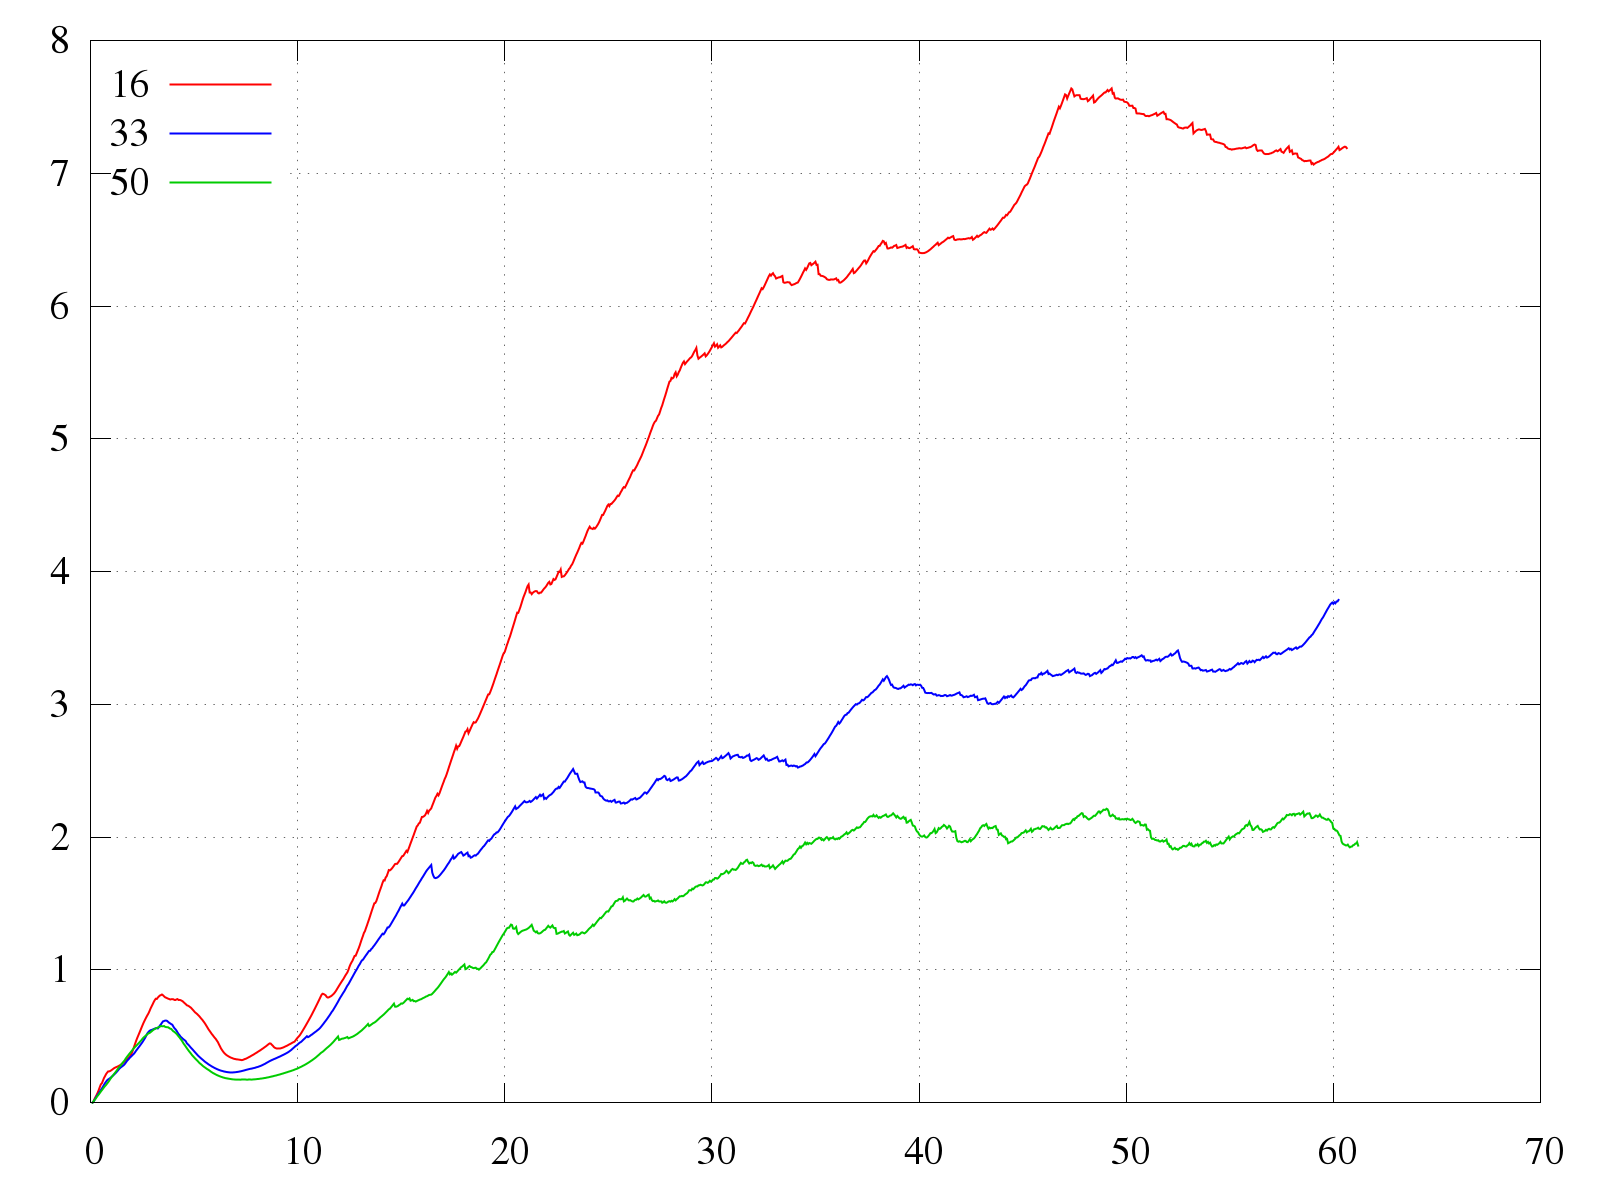
\includegraphics[width=.9\linewidth]{all_serial_ts.png}
    \caption{Равномерное распределение, 3 эксперимента, интервал обновления от времени}
    \label{fig:all_serial_ts}
\end{figure}

Из графика на рисунке \ref{fig:all_serial_pk} можно сказать, что скорость
разведывания карты не сильно отличается для 16, 33 и 50 юнитов. Но на
графике \ref{fig:all_serial_ts} можно видеть сильное различие в средней
актуальности карты для разных количеств юнитов.

\clearpage
\newpage

\subsubsection{Сравнение алгоритмов}

Рассмотрим работу различных вариаций алгоритмов с одинаковым количеством
юнитов.

\textbf{Работа с 16 юнитами}

\begin{figure}[h!]
    \centering
    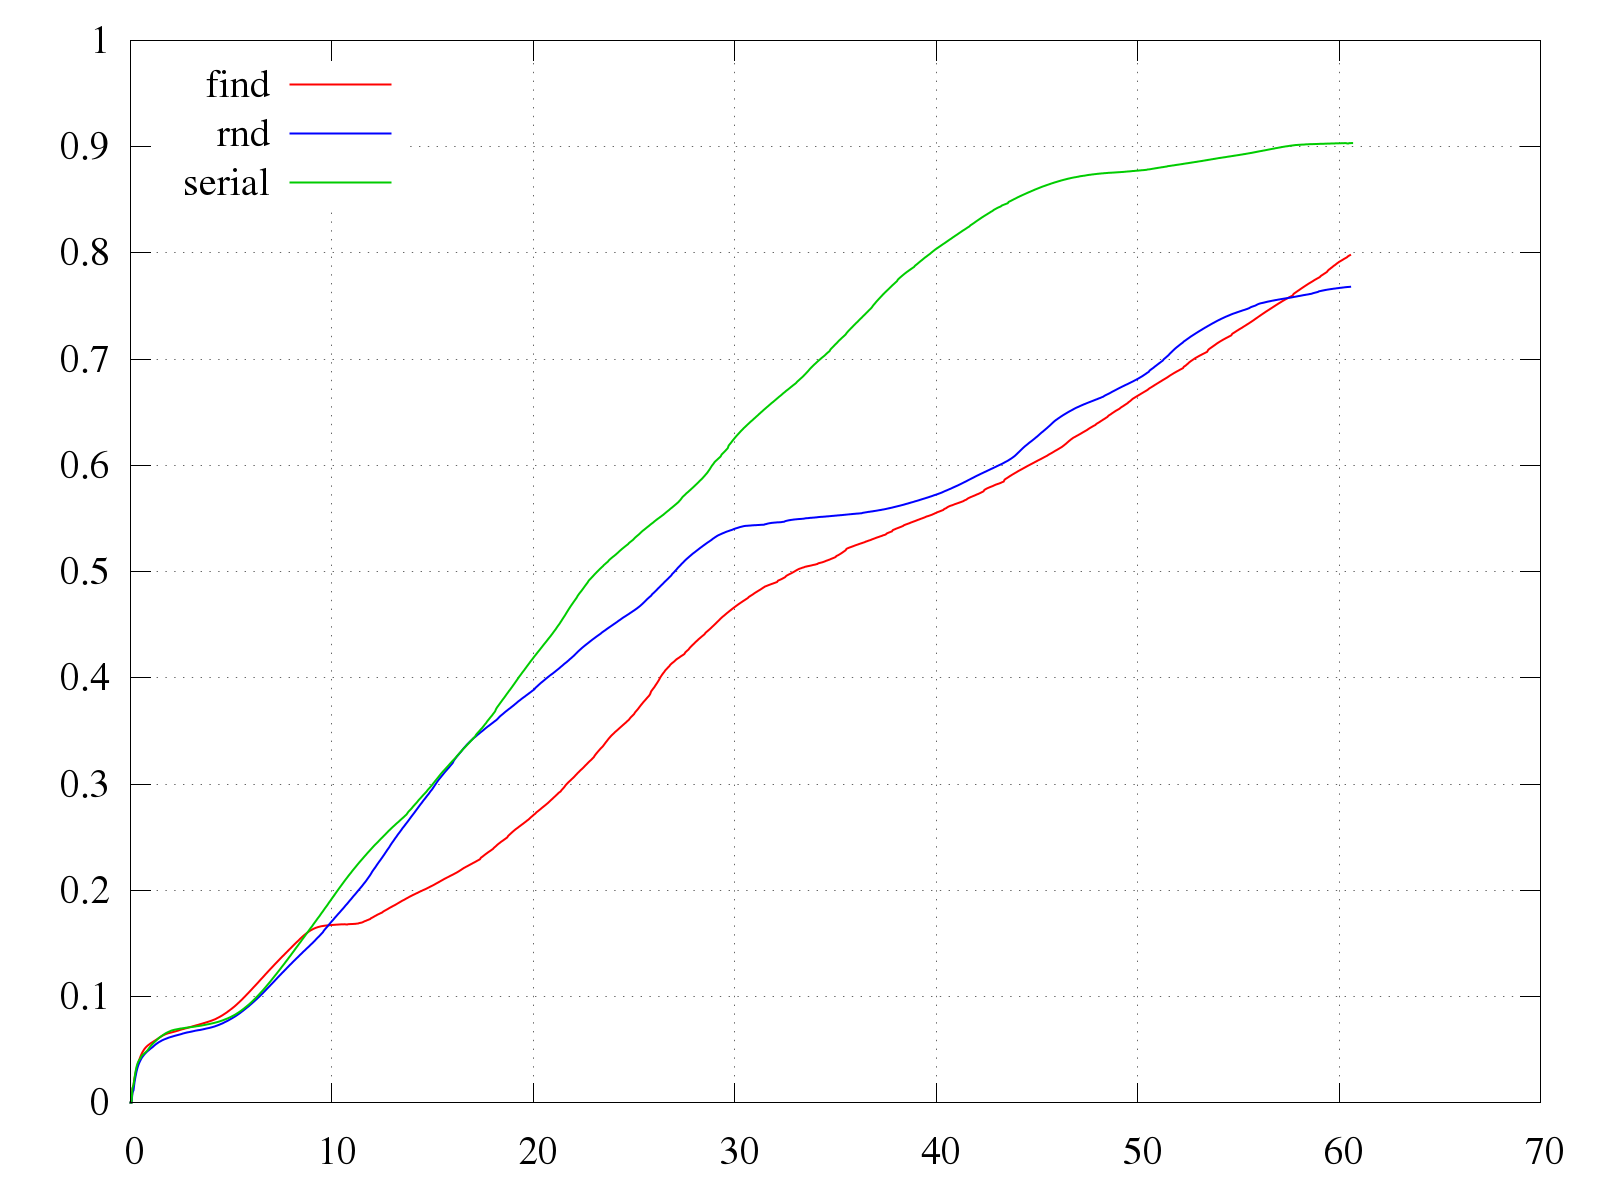
\includegraphics[width=.9\linewidth]{all_16_pknown.png}
    \caption{3 варианта, 16 юнитов, количество изведанных секторов от времени}
    \label{fig:all_16_pk}
\end{figure}

Из графика на рисунке \ref{fig:all_16_pk} можно видеть что хуже всех показывает
себя вариация алгоритма поиска ближайших неизведанных зон. Но различие между
вариацией со случайным выставлением целевой точки и поиском ближайших неизведанных
зон на 40-ой секунде симуляции становится незначительным. Равномерное распределение
юнитов по объёму карты показывает стабильный рост количества изведанных секторов
вплоть до 45-ой секунды симуляции.

\begin{figure}[h!]
    \centering
    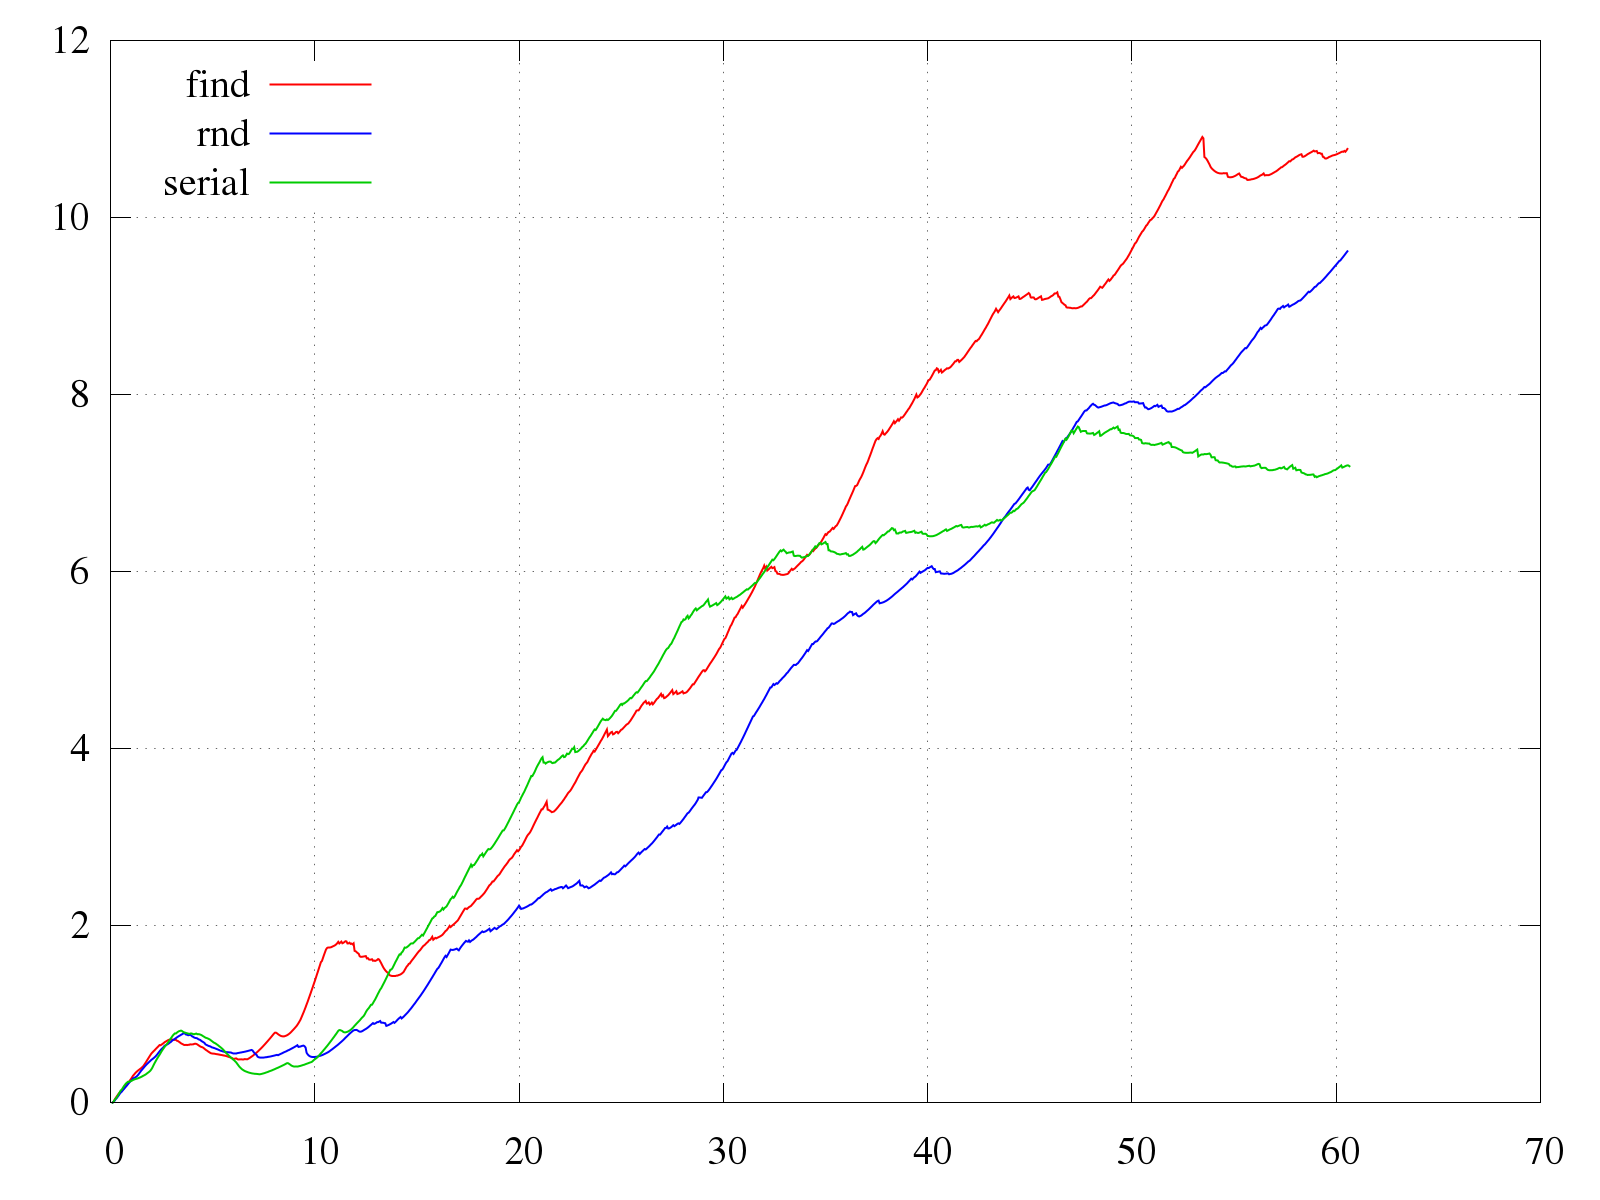
\includegraphics[width=.9\linewidth]{all_16_ts.png}
    \caption{3 варианта, 16 юнитов, интервал обновления от времени}
    \label{fig:all_16_ts}
\end{figure}

\newpage
При количестве в 16 юнитов каждая из вариаций алгоритма плохо показывает себя
в вопросе обновления карты. Но так же можно сказать, что хуже себя показал
алгоритм поиска ближайших неизведанных зон. График среднего интервала обновления
секторов для 16 юнитов показан на рисунке \ref{fig:all_16_ts}.

\clearpage
\newpage

\textbf{Работа с 33 юнитами}

\begin{figure}[h!]
    \centering
    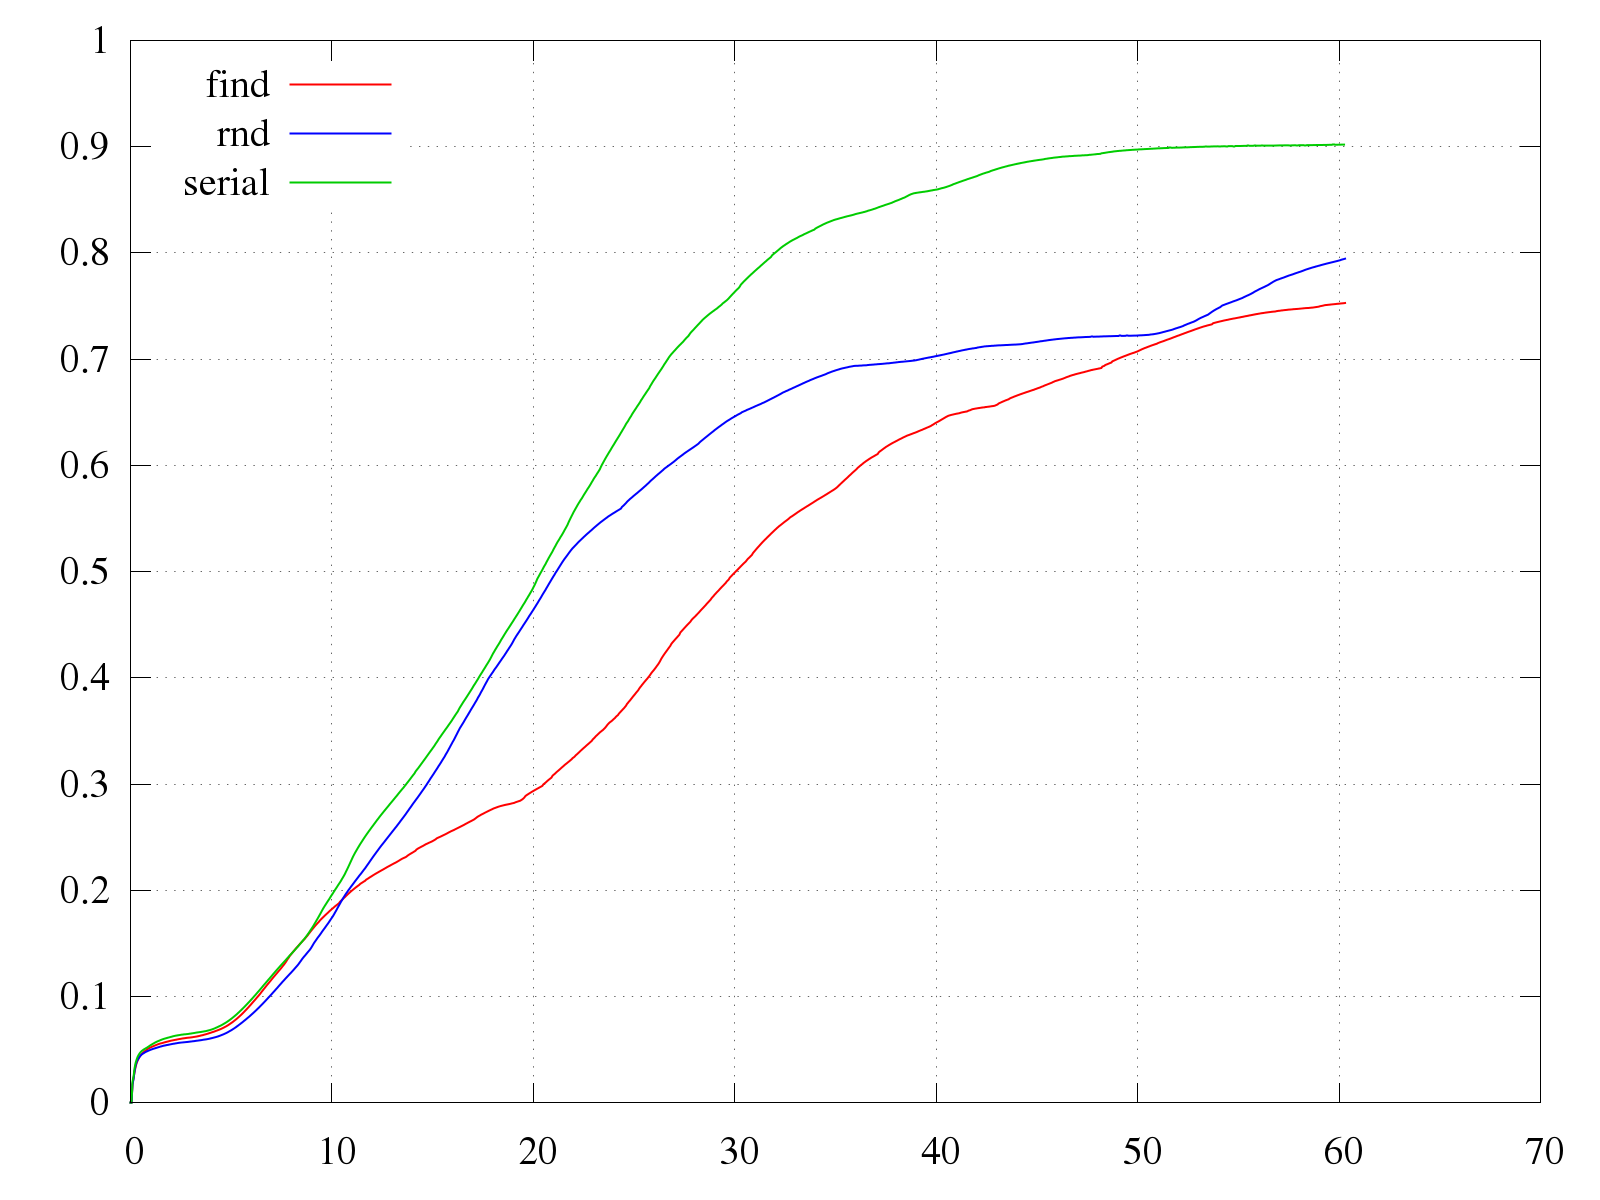
\includegraphics[width=.9\linewidth]{all_33_pknown.png}
    \caption{3 варианта, 33 юнита, количество изведанных секторов от времени}
    \label{fig:all_33_pk}
\end{figure}

Рассмотрим график на риунке \ref{fig:all_33_pk}
При работе с 33 юнитами можно заметить, что объем и скорость обследования
карты до 20 секунды симуляции почти не различаются у вариаций со случайным
выставлением целевой точки и равномерным распределением по регионам. Это
Можно объяснять тем, что перемещение юнитов начинается из центра и на
начальных этапах перемещение юнитов для этих вариаций выглядит практически
одинаково.

\begin{figure}[h!]
    \centering
    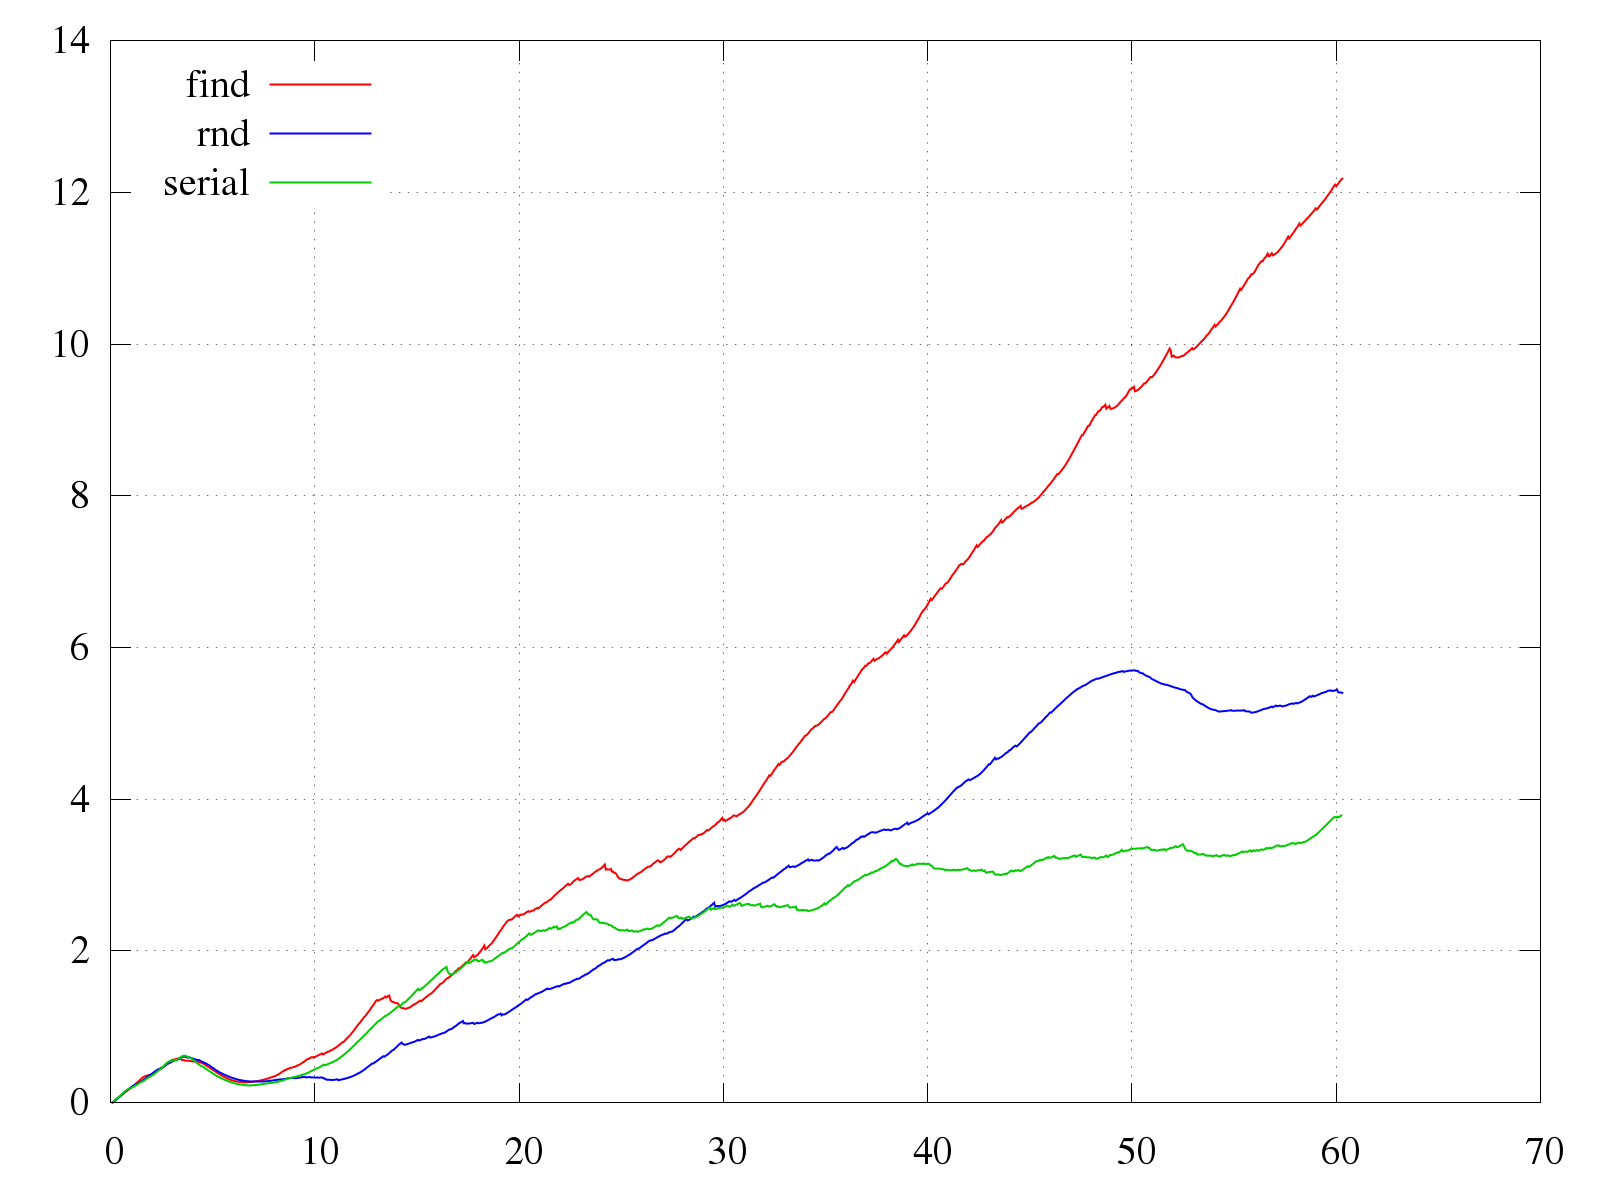
\includegraphics[width=.9\linewidth]{all_33_ts.png}
    \caption{3 варианта, 33 юнита, интервал обновления от времени}
    \label{fig:all_33_ts}
\end{figure}

\newpage
Так же на рисунке \ref{fig:all_33_ts} можно видеть как на 30 секунде вариация
алгоритма с равномерным распределением юнитов по регионам начинает показывать
более лучший результат по сравнению с алгоритмом случайного выставления целевой
точки. Как раз в этот момент времени становятся хорошо заметны различия маршрутов
между этими двумя вариациями. 

Алгоритм поиска ближайшей неизведанной зоны и при количестве в 33 юнита показывает
худший результат. Стабильный рост "устаревания" секторов для этой вариации
алгоритма обословлен тем, что юниты скапливаются в определённых регионах и не
выходят оттуда. Это связанно с тем, что каждый раз, когда выбирается регион
с наибольшим количеством неизведанных секторов он попадает в область внутри
здания, куда юниты не могут попасть.

\clearpage
\newpage

\textbf{Работа с 50 юнитами}

При количестве юнитов в 50 единиц мы видим схожую картину, что и при 33 юнитах.
Для вариации со случайным выставлением целевой точки можно наблюдать
тенденцию перерастания количества в качество.

\begin{figure}[h!]
    \centering
    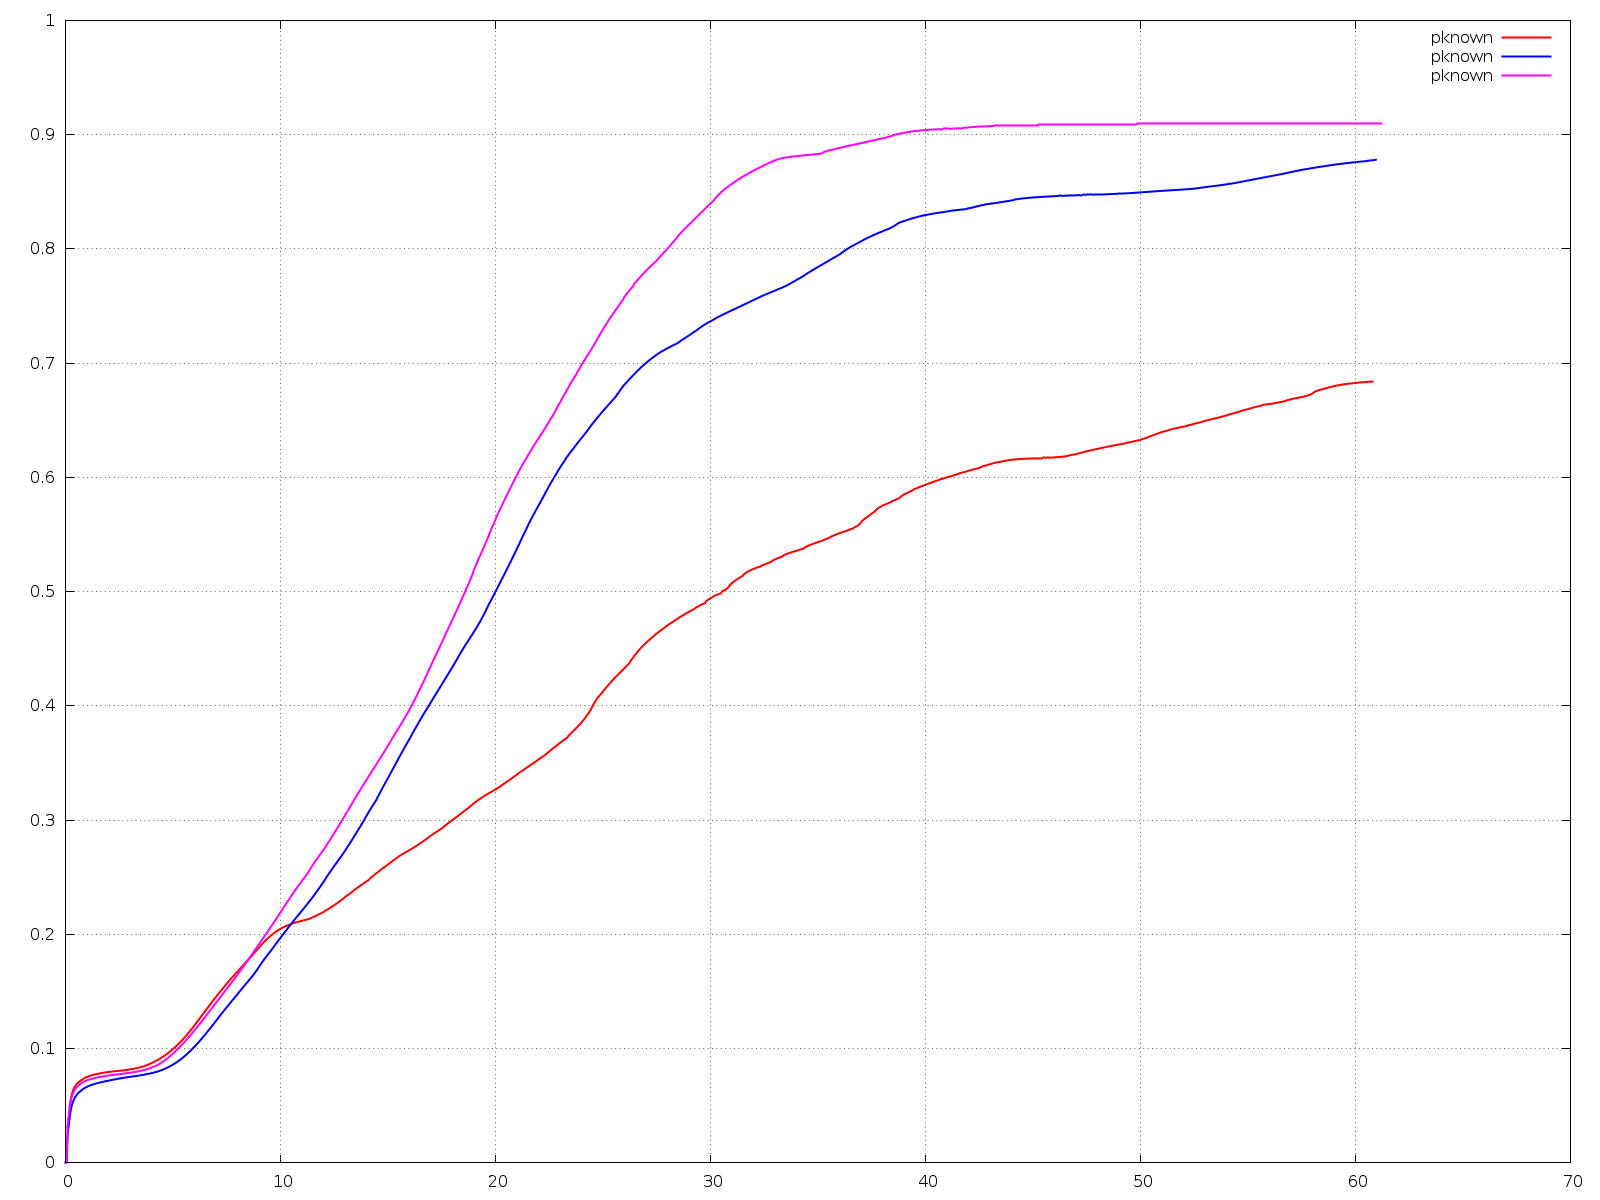
\includegraphics[width=.8\linewidth]{all_50_pknown.png}
    \caption{3 варианта, 50 юнитов, количество изведанных секторов от времени}
    \label{fig:all_50_pk}
\end{figure}

\begin{figure}[h!]
    \centering
    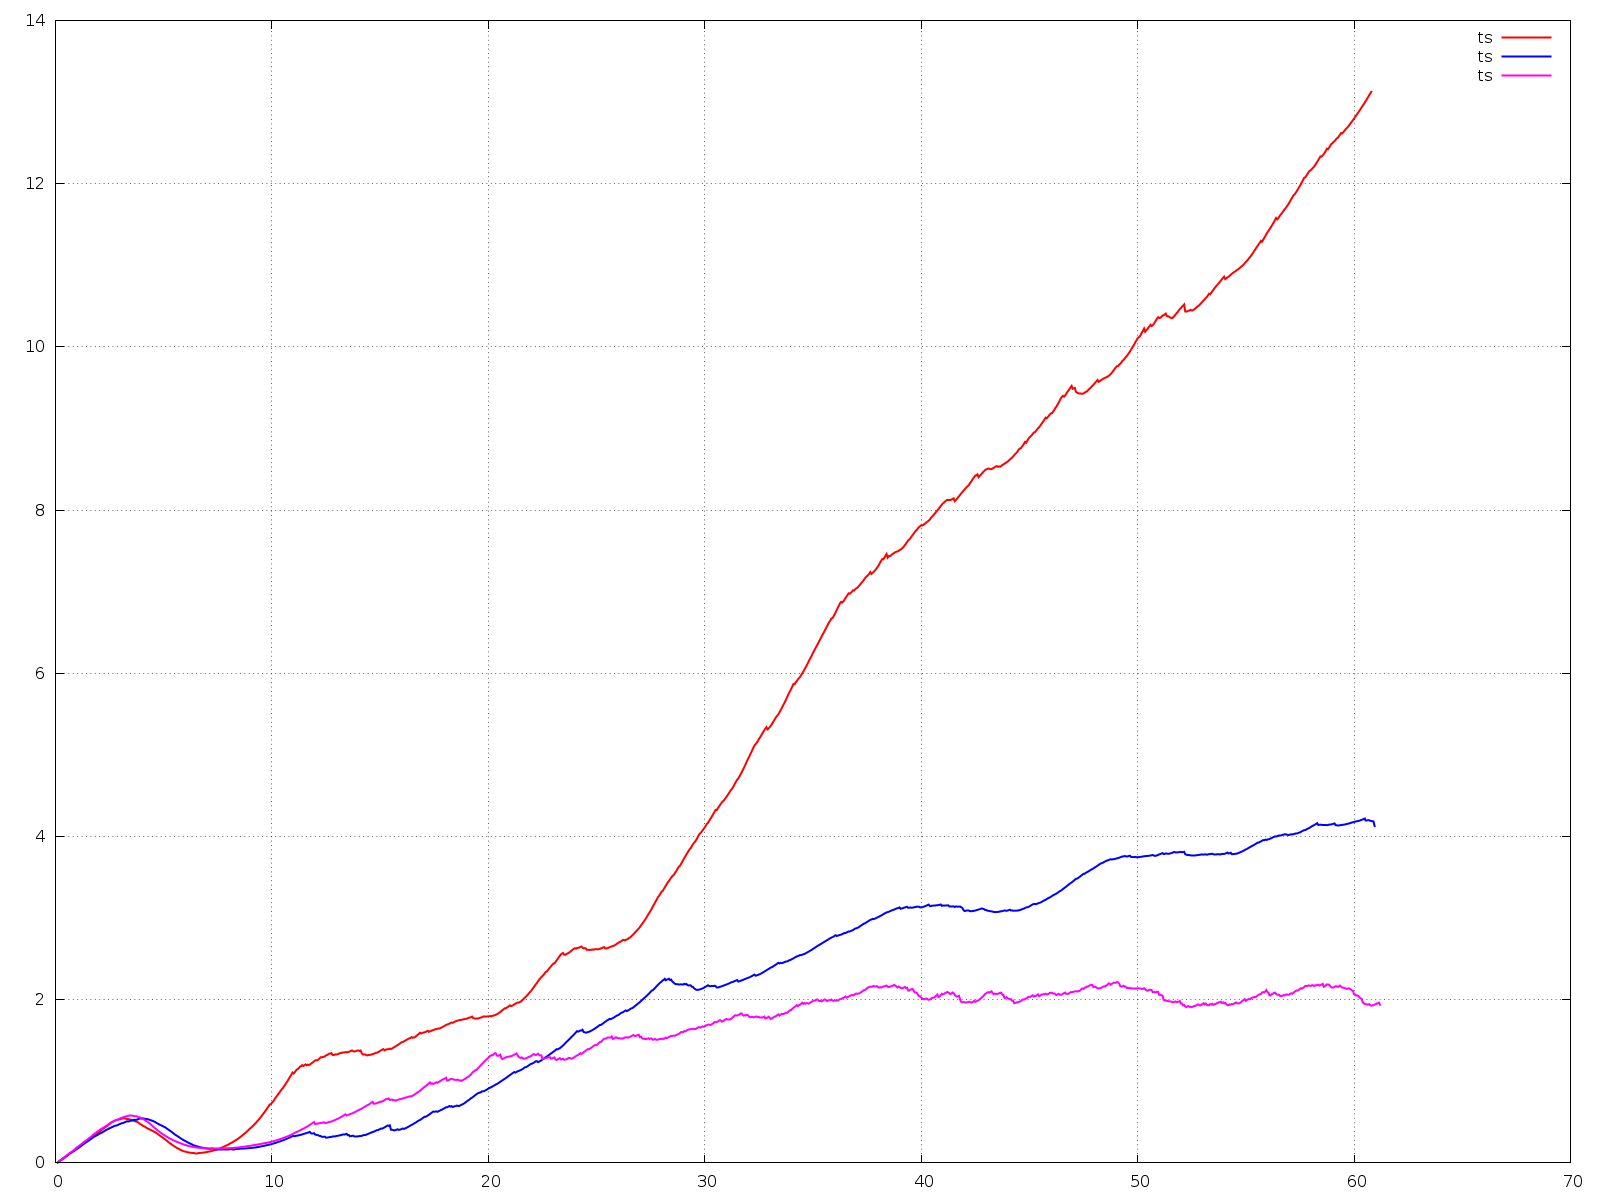
\includegraphics[width=.8\linewidth]{all_50_ts.png}
    \caption{3 варианта, 50 юнитов, интервал обновления от времени}
    \label{fig:all_50_ts}
\end{figure}

\clearpage
\newpage

\textbf{Общее сравнение и анализ}

Приведём графики для всех 9 экспериментов.

\begin{figure}[h!]
    \centering
    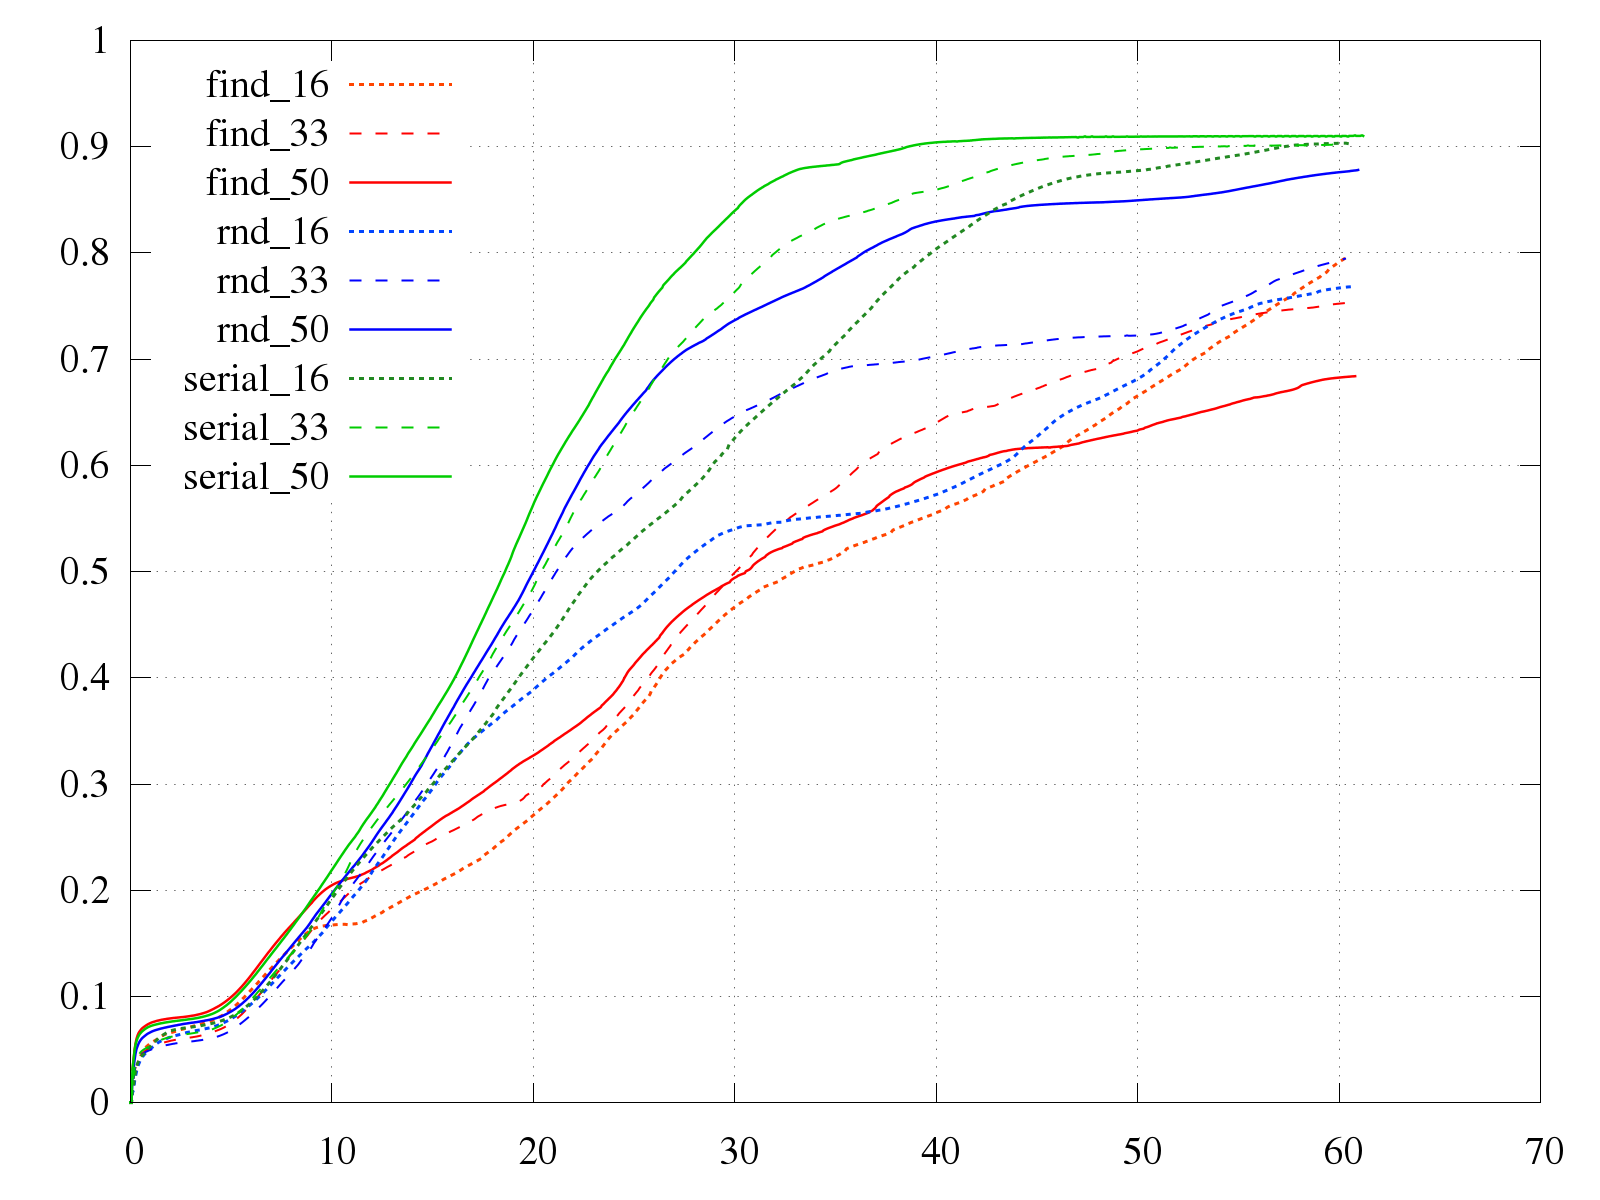
\includegraphics[width=.9\linewidth]{all_pknown.png}
    \caption{3 варианта, 50 юнитов, количество изведанных секторов от времени}
    \label{fig:all_pk}
\end{figure}

Из графика на рисунке \ref{fig:all_pk} можно заметить, что для алгоритма
равномерного распределения по регионам карты при количесвах 33 и 50 юнитов
разница результатов не существенна, хотя для алгоритма случайного выставления
целевой точки она гораздо больше. Но алгоритм равномерного распределения
приходит к значению 0.9 даже при количестве в 16 юнитов. Это связанно с тем,
что 16 это количество регионов карты, между которыми происходит распределение
юнитов. Каждый юнит обследует свою область. Из рисунка \ref{fig:s50s_map2} 
можно понять, почему ни один из алгоритмов не набрал значение обследования
больше 0.9: 10\% карты занимают здания, в которые юниты не могут залетать.

\begin{figure}[h!]
    \centering
    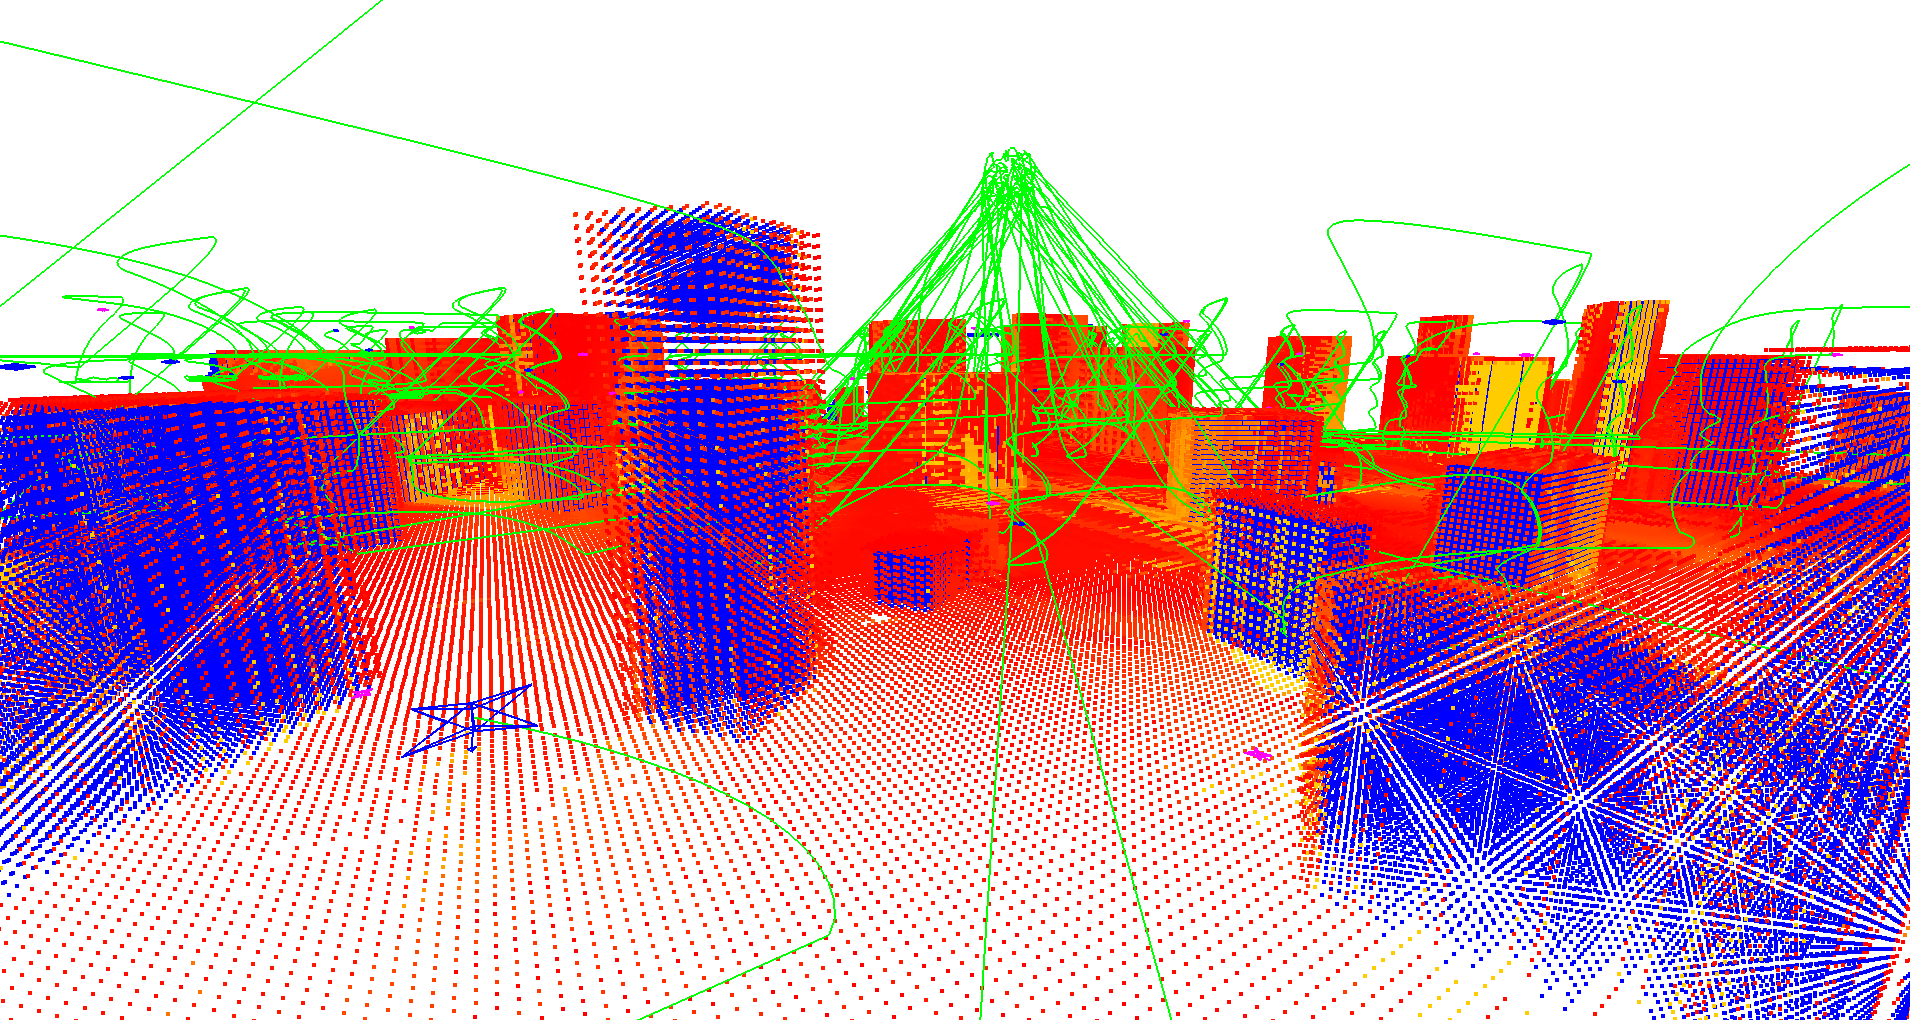
\includegraphics[width=.9\linewidth]{s50s_map2.png}
    \caption{Равномерное распределение, 50 юнитов, вид сбоку, состояние карты}
    \label{fig:s50s_map2}
\end{figure}

\begin{figure}[h!]
    \centering
    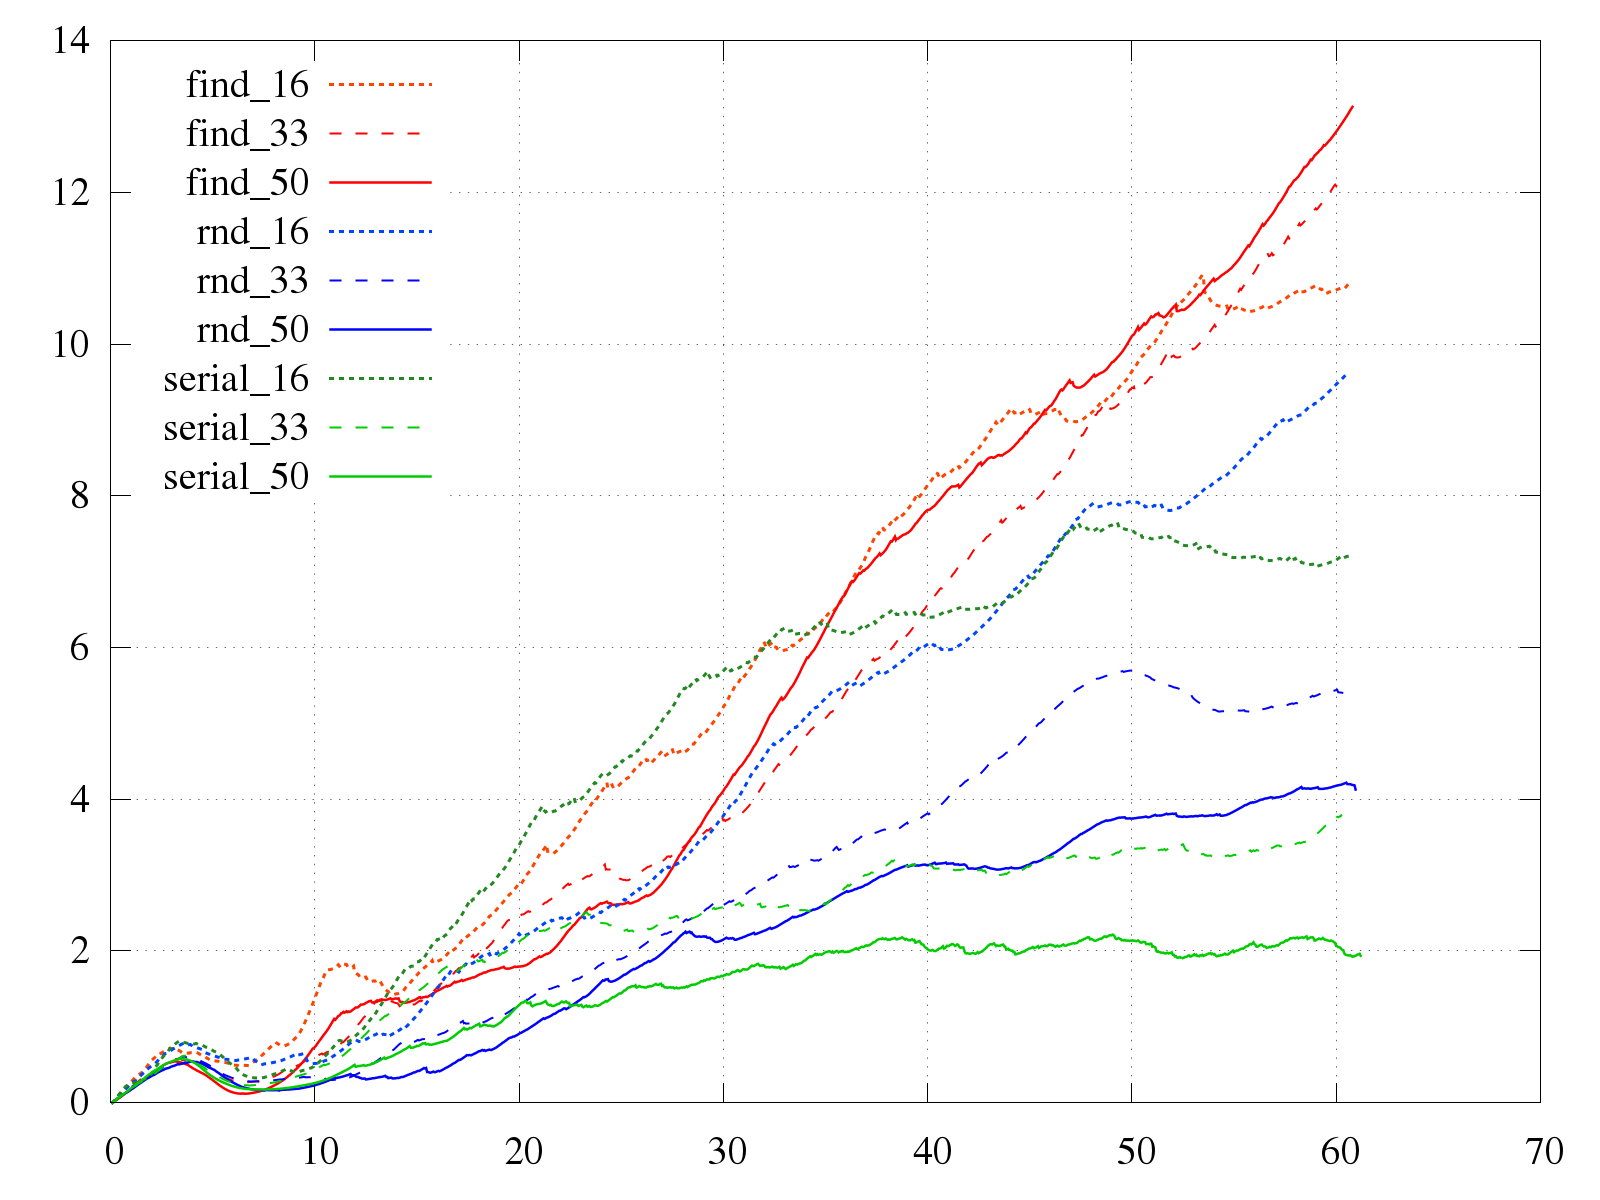
\includegraphics[width=.9\linewidth]{all_ts.png}
    \caption{3 варианта, 50 юнитов, интервал обновления от времени}
    \label{fig:all_ts}
\end{figure}

Для задачи обновления карты можно определить правило: чем больше юнитов, тем
лучше. Это хорошо заметно на рисунке \ref{fig:all_ts} при рассмотрении
алгоритмов случайного выставления целевой точки и для равномерного распределения
по регионам. На них практически одинаково повлияло увеличение количества юнитов.

\clearpage

\subsubsection{Выводы}

На удивление хорошо себя показала вариация алгоритма обследования местности
со случайным выставлением целевой точки. Это можно объяснить структурой карты:
все объекты представляют из себя паралелограммы, без внутренней структуры.
Лучше всех показал себя алгоритм более детерминированного характера:
равномерное распределение по регионам карты.

Алгоритм поиска неизведанных секторов оказался недоработанным. В него следует
включить некоторые изменения: проверка доступности целеой точки. Эта задача
достаточно сложна вычислительно.

Обратим внимание на схожее поведение алгоритмов в начале симуляции, вплоть до
10 секунды. Это связанно с тем, что юниты появляются в точке над центром карты
и начинают своё движение вниз и в стороны для каждой вариации алгоритма.
С этим же связанно сокращение среднего интервала обновления к 8ой секунде:
юниты, двигаясь от стартовой точки смотрят в направлении скорости и к этому
времени достаточно мало объёма исследованно, а тот что исследован находится
в области обзора камер юнитов.

В итоге хочется сказать, что эксперименты проводились в определённых
условиях, при смене которых нельзя гарантировать подобное поведение
алгоритмов.

\clearpage
\newpage
